% Autor: Jakub Sadílek 2020
%=========================================================================
\chapter{Úvod}
Náplní této práce je zpřístupnit nástroj pro pokročilou filtraci textu běžným uživatelům. Filtraci textových dat lze řešit v~IT oblasti různými nástroji. Ovšem lidé neznalí programování tuto situaci musí řešit komplikovaným způsobem nebo využít již dostupná řešení, která jim alespoň zčásti pomohou. Větší problém pak nastává při složitější transformaci, kterou nelze vyřešit elementární operací.

V současné době existují na internetu různé nástroje řešící tento problém, které využije i~znalý programátor kvůli jejich snadné dostupnosti, ale poskytují jen jednu operaci najednou, tudíž je potřeba text neustále kopírovat nebo v~horším případě hledat jiné stránky poskytující právě požadovanou operaci. Na otázku \uv{Jak se tento záznam na onom řádku promítl do výsledku?} se odpověď hledá jen těžko. Pokud by někdy v~budoucnu bylo potřeba provést transformaci znovu, je nutné celý proces opakovat a~to stojí čas.

Hlavní motivací této práce je eliminovat výše uvedené nedostatky a~poskytnout uživatelům komplexní nástroj s~velkou variabilitou, ve kterém mohou snadno a~efektivně sestavit výslednou podobu textu s~možností prototypování a~ladění. Nabídnout uživatelům aplikaci, ve které mohou odfiltrovat nepodstatné informace například z~textových tabulek, zpracovat log soubory, a~to vše naráz z~jednoho místa.

V následujícím textu je podrobněji obsažena většina aspektů, které bylo potřeba při vývoji řešit. Přesněji v~kapitole~\ref{chap:Zpracování textových dat a současný stav} je zmíněna problematika filtrování, proč má smysl data filtrovat a~jsou zde představeny existující nástroje. Kapitola~\ref{chap:Návrh webové aplikace} obsahuje proces návrhu, zpracování požadavků na aplikaci, kritéria pro výběr nástrojů a~nakonec je zmíněna cílová skupina uživatelů. Kapitola~\ref{chap:Použité technologie} se zaměřuje na nejpodstatnější technologie použité v~aplikaci a~hlouběji je popsán jejich princip a~funkčnost. V kapitole~\ref{chap:Implementace webové aplikace} o~implementaci je popsána dekompozice a~struktura projektu, jak probíhá proces zpracování a~ukazuje zajímavé části kódu. Závěr této kapitoly obsahuje ukázky výsledné aplikace. Poslední kapitola~\ref{chap:Sběr dat a testování} se věnuje sběru testovacích dat, automatizovanému a~uživatelskému testování včetně vyhodnocení.

%=========================================================================
\chapter{Zpracování textových dat a současný stav}
\label{chap:Zpracování textových dat a současný stav}
První část této kapitoly uvede čtenáře do problematiky zpracování textových souborů. Jsou zde popsány situace, kde se s~touto problematikou setkáváme a~jak vzniká. Druhá část kapitoly je věnována dostupným řešením, které lze v~dnešní době použít včetně dostupných aplikací na internetu.

\section{Problematika zpracování textových souborů}
Řešit tento problém v~IT průmyslu je běžnou praxí. Správci sítě se s~ním potýkají například při analýze přístupových logů, systémoví administrátoři v~operačních systémech nebo programátoři, jejichž programy na těchto datech závisí. Běžní uživatelé se s~takovými daty mohou setkat při jednoduše překopírovaných tabulkách, v~publikovaných seznamech nebo soupiskách či jinde. Také existují portály, které zveřejňují zajímavé datové sady z~oblasti výzkumů jako například Kaggle\footnote{Kaggle: \url{https://www.kaggle.com}}. Typicky jsou tato data rozsáhlá a~jejich zpracování bez použití automatizace je časově náročné. 

Odhadem při 300 a~více záznamech nastává situace vhodná k~použití automatizovaných nástrojů. Obzvlášť pokud se jedná o~neseřazená data. Nejčastější operací bývá vyhledávání, které lze snadno provést klávesovou zkratkou \uv{ctrl + F} implementovanou ve většině prohlížečích. Pokud je potřeba data uložit, přeposlat nebo zveřejnit je vhodné odstranit nepodstatné informace a~tím text modifikovat. Odstranění záznamu lze provést snadno odstraněním příslušného řádku v~případě malého počtu, ale při odstranění, modifikaci informace v~záznamu \textit{(tj.~sloupce)} nebo řazení nastává situace komplikovanější, jelikož musíme upravit každý jednotlivý záznam zvlášť.

\section{Řešení v dnešní době}
V dnešní době existuje celá škála možností jak z~textu vyfiltrovat podstatné informace. Jedním ze způsobů je vytvořit si jednoduchý program nebo skript. Programátor vytvoří algoritmus, který realizuje transformaci a~ten naprogramuje v~libovolném jazyku. Dnes se může jednat o~Python, PHP, Bash, JavaScript a~mnoho dalších. Nevýhoda tohoto způsobu je, že čas strávený při implementaci může být zbytečně dlouhý a~silně závisí na dovednostech dané osoby, obzvlášť pokud jde o~jednorázovou filtraci a~program pak zůstane nevyužitý. V opačném případě je toto řešení velmi efektivní.

Co když jedinec není programátor? Pak nejspíše využije některých z~nástrojů, které jsou zdarma snadno dostupné, nejspíše na webu. To je druhý způsob, kterým lze problém řešit. Tyto nástroje fungují na podobném principu: vložit vstupní text, provést operaci a~vyjmout výsledek. Takových nástrojů existuje na internetu celá řada, následně si uvedeme příklad těch nejzajímavějších.

\subsection*{Online text tools}
Online text tools\footnote{Online text tools: \url{https://onlinetexttools.com}} je populární webová stránka pro zpracování textu, která nabízí velké množství nástrojů a~v~budoucnu plánuje přidat ještě další. Nabízí také vyhledávač, který umožňuje přehledně redukovat výběr nástrojů. Část stránky je znázorněna na obrázku~\ref{obr:Online text tools}. Jak je na samotné stránce uvedeno, funguje na principu \uv{načíst text, získat výsledek}.
\begin{figure}[hbt]
	\centering
	\setlength{\fboxsep}{0pt}
	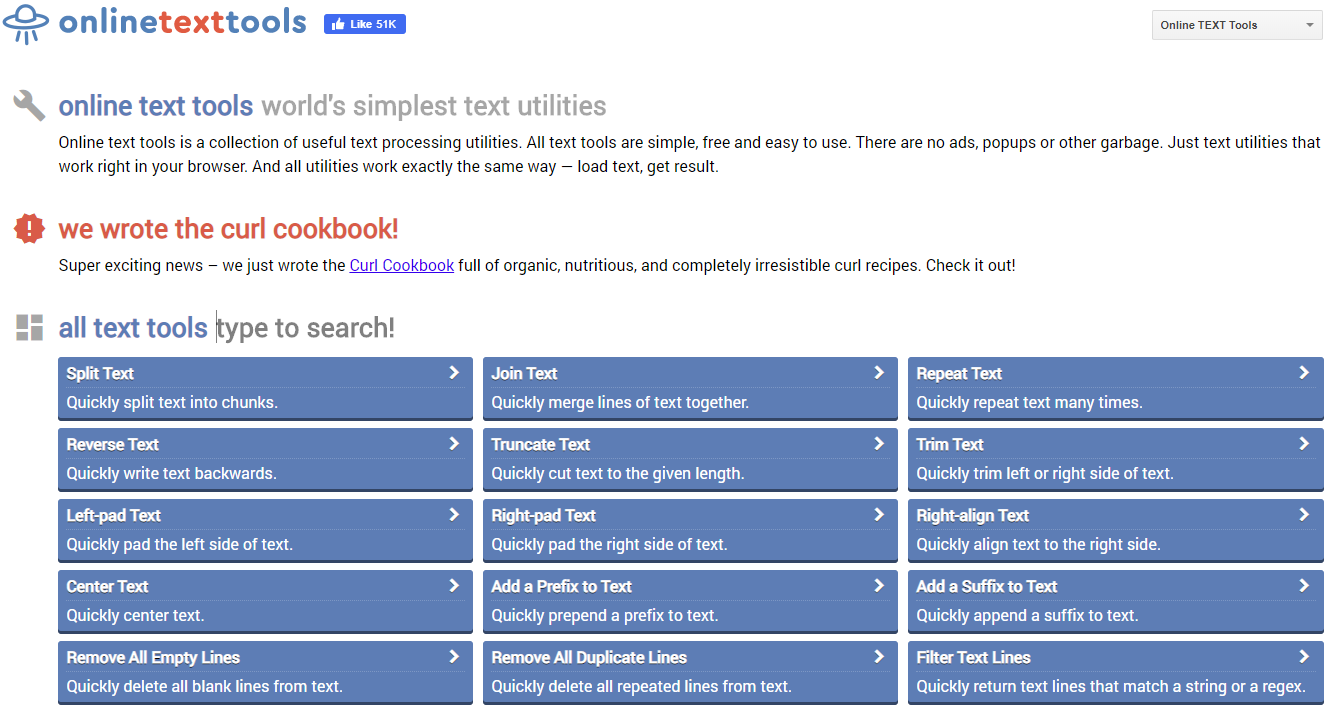
\includegraphics[width=1\textwidth]{obrazky-figures/onlinetexttools_prehled.png}
	\caption{Ukázka úseku hlavní stránky aplikace online text tools, na které je zobrazena část nabízených nástrojů.}
	\label{obr:Online text tools}
\end{figure}

\subsection*{Browserling}
Browserling\footnote{Browserling: \url{https://www.browserling.com/tools}} je další zajímavý webový portál, který nabízí spoustu nástrojů, které zejména ocení vývojáři webových stránek. V nabídce jsou nástroje pro práci s~obrázky, časem, šifrováním a~další. My se zaměříme pouze na ty textové.

Celkem je obsaženo $113$~textových funkcí, které lze použít, ovšem většina je velmi specifická, a~tak mají jen velmi úzké spektrum využití jako například převody mezi kódováním nebo datovými formáty. Nástroje fungují také na principu vstup, jednoduchá operace a~výstup. Přes velkou kolekci nástrojů si tu každý najde svoji podmnožinu, která se mu hodí. Náhled úseku stránky je zobrazen na obrázku~\ref{obr:Browserling}.
\begin{figure}[hbt]
	\centering
	\setlength{\fboxsep}{0pt}
	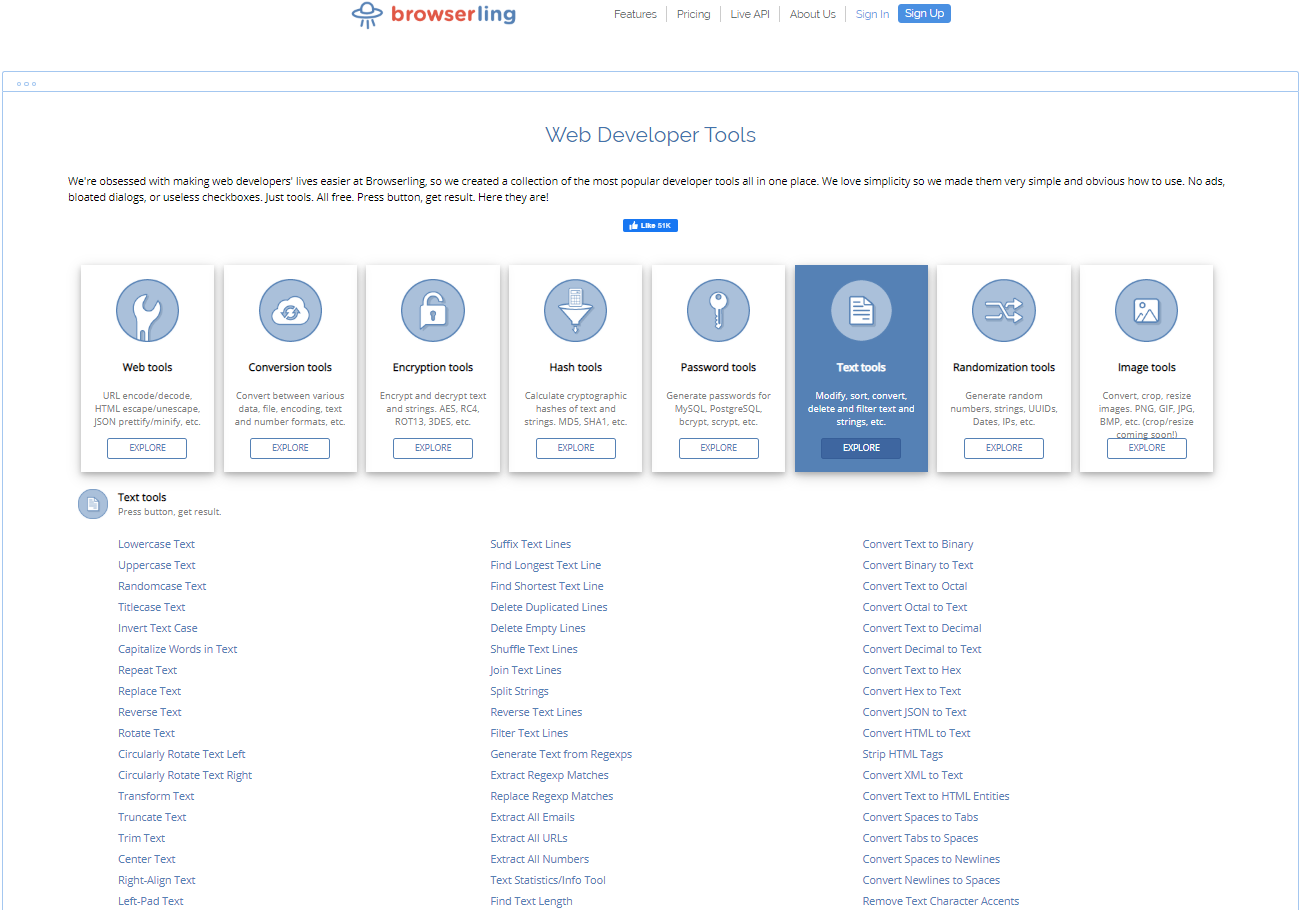
\includegraphics[width=1\textwidth]{obrazky-figures/browserling_prehled.png}
	\caption{Ukázka části galerie s~textovými nástroji webové aplikace Browserling.}
	\label{obr:Browserling}
\end{figure}

\subsection*{Zhodnocení existujících řešení}
V existujících testovaných aplikacích lze provést pouze jednu operaci v~daný okamžik a~při dalším zpracování je nutné hledat potřebnou funkci jinde. Některé aplikace neumožňují nahrát vstupní text ze souboru či stáhnout výsledek. Velikost vstupních elementů bývá malá a~při obsáhlejších datech způsobuje nepřehlednost a~ztěžuje orientaci v~textu, zároveň aplikace neposkytují podpůrné funkce, které usnadňují dodatečnou manipulaci se vstupním textem. Většinou také galerie nebývají nijak členěny a~nástroje jsou zobrazeny pouze v~jednoduchém seznamu. Možnost prototypování nenabízela žádná z~testovaných aplikací, a~když si ke konci filtrace uživatel uvědomí, že ve výsledku opomněl některé záznamy, musí celý proces provést znovu.

U výše testovaných aplikací je velkou výhodu, že nabízí velkou rozmanitost nástrojů, proto hledání jiných služeb realizující požadovanou operaci nastává výjimečně a~obsah těchto galerií byl inspirací při návrhu implementovaného řešení.

%=========================================================================
\chapter{Návrh webové aplikace}
\label{chap:Návrh webové aplikace}

Tato kapitola obsahuje celý proces návrhu aplikace. Jsou zde zmíněny původní záměry a~řešení, které poskytuje a~rozebrán vývoj uživatelského rozhraní. Další část kapitoly je zaměřena na výběr nástrojů, které byly v~aplikaci implementovány. Na závěr je uvedeno na koho aplikace cílí a~kdo by mohl být typickým uživatelem.

\section{Požadavky na webovou aplikaci}
\label{sec:Požadavky na webovou aplikaci}
Hlavním požadavkem na aplikaci je nabídnout uživateli nástroj, ve kterém lze snadno a~efektivně vyfiltrovat podstatné informace z~textových dat. Taková filtrace může obsahovat složitou transformaci, kterou je možné sestavit ze sekvence jednodušších, elementárních operací. Proces zpracování je pak možné realizovat pomocí zřetězeného zpracování (pipelining), kde výstup operace poskytne vstup následující operaci. Mezi další požadavky patří:

\subsection*{Komfortní editor}
Použity jsou celkem dva editory, jeden je určen pro vstup, druhý zobrazuje výsledek a~je určen pouze ke čtení. Editor je základ celé aplikace, proto by měl nabízet také mnoho funkcí, které uživateli usnadní práci. Zejména se může jednat o~práci se soubory, které ušetří některé nadbytečné úkony nebo o~hromadné akce, které by musel uživatel jednotlivě a~opakovaně provádět. S~větším počtem uživatelů může také vzniknout více požadavků na operace se vstupními daty nebo jejich zobrazení. Implementované funkce do editoru tedy jsou:
\begin{itemize}
    \item Manipulace se soubory
    \item Zpětné a~dopředné vracení změn
    \item Zalamování textu
    \item Ovládání režimu
    \item Hromadné ovládání použitých nástrojů
    \item Vyhledávač v~textu včetně regulárních výrazů
\end{itemize}

\subsection*{Intuitivní a jednoduché rozhraní}
Při tvorbě takového rozhraní je zapotřebí spousta testování, protože aplikace je určena pro široké spektrum uživatelů, musí rozhraní vyhovovat všem. Typicky náročnost použití rozhodne o~tom, jak bude výsledek oblíbený. Uživatel musí intuitivně tušit kam se podívat a~co kde hledat při jeho úkonech. Více o~návrhu uživatelského rozhraní lze nalézt v~následující kapitole~\ref{sec:Uživatelské rozhraní}, výsledná podoba je pak znázorněna v~kapitole~\ref{sec:Výsledná podoba aplikace}.

\subsection*{Eliminace zbytečných úkonů}
Tuto vlastnost můžeme pozorovat například při zpracovávání textu pomocí shellu, ze kterého byla převzata inspirace v~mnoha směrech. Prakticky může stačit pouze jeden výraz k~dosáhnutí výsledné podoby textu. Takto lze ušetřit zbytečné operace jako je překopírování, přesměrování stránek a~nabídnout vše na jednom místě. Tento způsob je poměrně originální a~žádná testovaná aplikace tuto možnost nenabízela.

\subsection*{Prototypování a ladění}
\uv{Moment, výběr klasickým výrazem nestačí, ale musím použít regulární výraz!} Nástroj lze jednoduše smazat nebo deaktivovat a~případně znovu použít později. Špatné pořadí operací? Lze jej kdykoliv zaměnit. 

\uv{Na vstupu mám $100\,000$~záznamů, a~právě tento záznam je pro mě poměrně důležitý. Jak se promítl do výsledku?} Stačí kliknout na odpovídající číslo řádku, kde se záznam nachází a~aplikace sama zobrazí jeho výslednou podobu včetně kontextu, ve kterém se nachází. To znamená, že pokud jsou použity nástroje, které zaměňují pořadí záznamu, pak ve výsledku při vyobrazení dvou a~více záznamů budou vůči sobě v~pozici, ve které se nachází ve výsledném textu. Tohle je další poměrně originální řešení, které nenabízí žádná z~testovaných aplikací.

\subsection*{Informovat uživatele}
\label{sec:Informovat uživatele}
Uživatel by měl být vždy informován o~tom, co právě provedl, co se v~aplikaci právě děje nebo v~jakém stavu se nachází. V aplikaci jsou proto implementovány různé funkce, které tuto situaci usnadňují.

Pro sdělující informace byla implementována vyskakující okna, která se zobrazují vlevo dole na monitoru a~sdělují informaci po provedení určitých akcí. Celkem byly zavedeny čtyři typy, a~to úspěšné (zelené), varovné (žluté), chybové (červené) a~oznamující (modré) pro okamžité rozeznání kontextu. Zároveň je důležité, aby se okno nezobrazovalo příliš často a~nestalo se tak pro uživatele obtěžující.

Další neméně důležitou vlastností je informovat uživatele o~aktuálním stavu procesu zpracování textu. Jelikož práce s~textovými řetězci je časově náročná operace, obzvlášť při velkém objemu dat, byla proto implementována načítající \textbf{deterministická} lišta, která vizuálně zobrazuje zbývající množství času, které je potřeba pro zpracování textu, aby uživatel nenabyl dojmu, že se nic neděje a~aplikace zamrzla nebo neodpovídá. Hrubým příkladem při $10\,000$~záznamech nelze změnu postřehnout, ovšem při $200\,000$ ji už lze zaznamenat. Především záleží na počtu znaků v~záznamu, náročnosti operace a~jejich počtu.

Všechny dostupné nástroje a~možnosti jsou doprovázeny popisky, které vysvětlují význam operace nebo fungování nástroje, a~tak by neměla nastat situace, kdy by uživatel nevěděl, co se bude dít. Tuto skutečnost potvrdilo i~testování, které se nachází v~kapitole~\ref{chap:Sběr dat a testování}.

O stavu editoru informuje spodní lišta, která zobrazuje:
\begin{itemize}
    \item Pozici kurzoru v~editoru
    \item Režim editoru
    \item Stav zalamování textu
\end{itemize}

\section{Uživatelské rozhraní}
\label{sec:Uživatelské rozhraní}
Na samotném začátku projektu byl vytvořen interaktivní prototyp aplikace (viz obrázek~\ref{obr:První návrh}) v~prostředí \textbf{AdobeXD}, na kterém byl demonstrován můj pohled na výsledný produkt.
\begin{figure}[hbt]
	\centering
	\setlength{\fboxsep}{0pt}
	\fbox{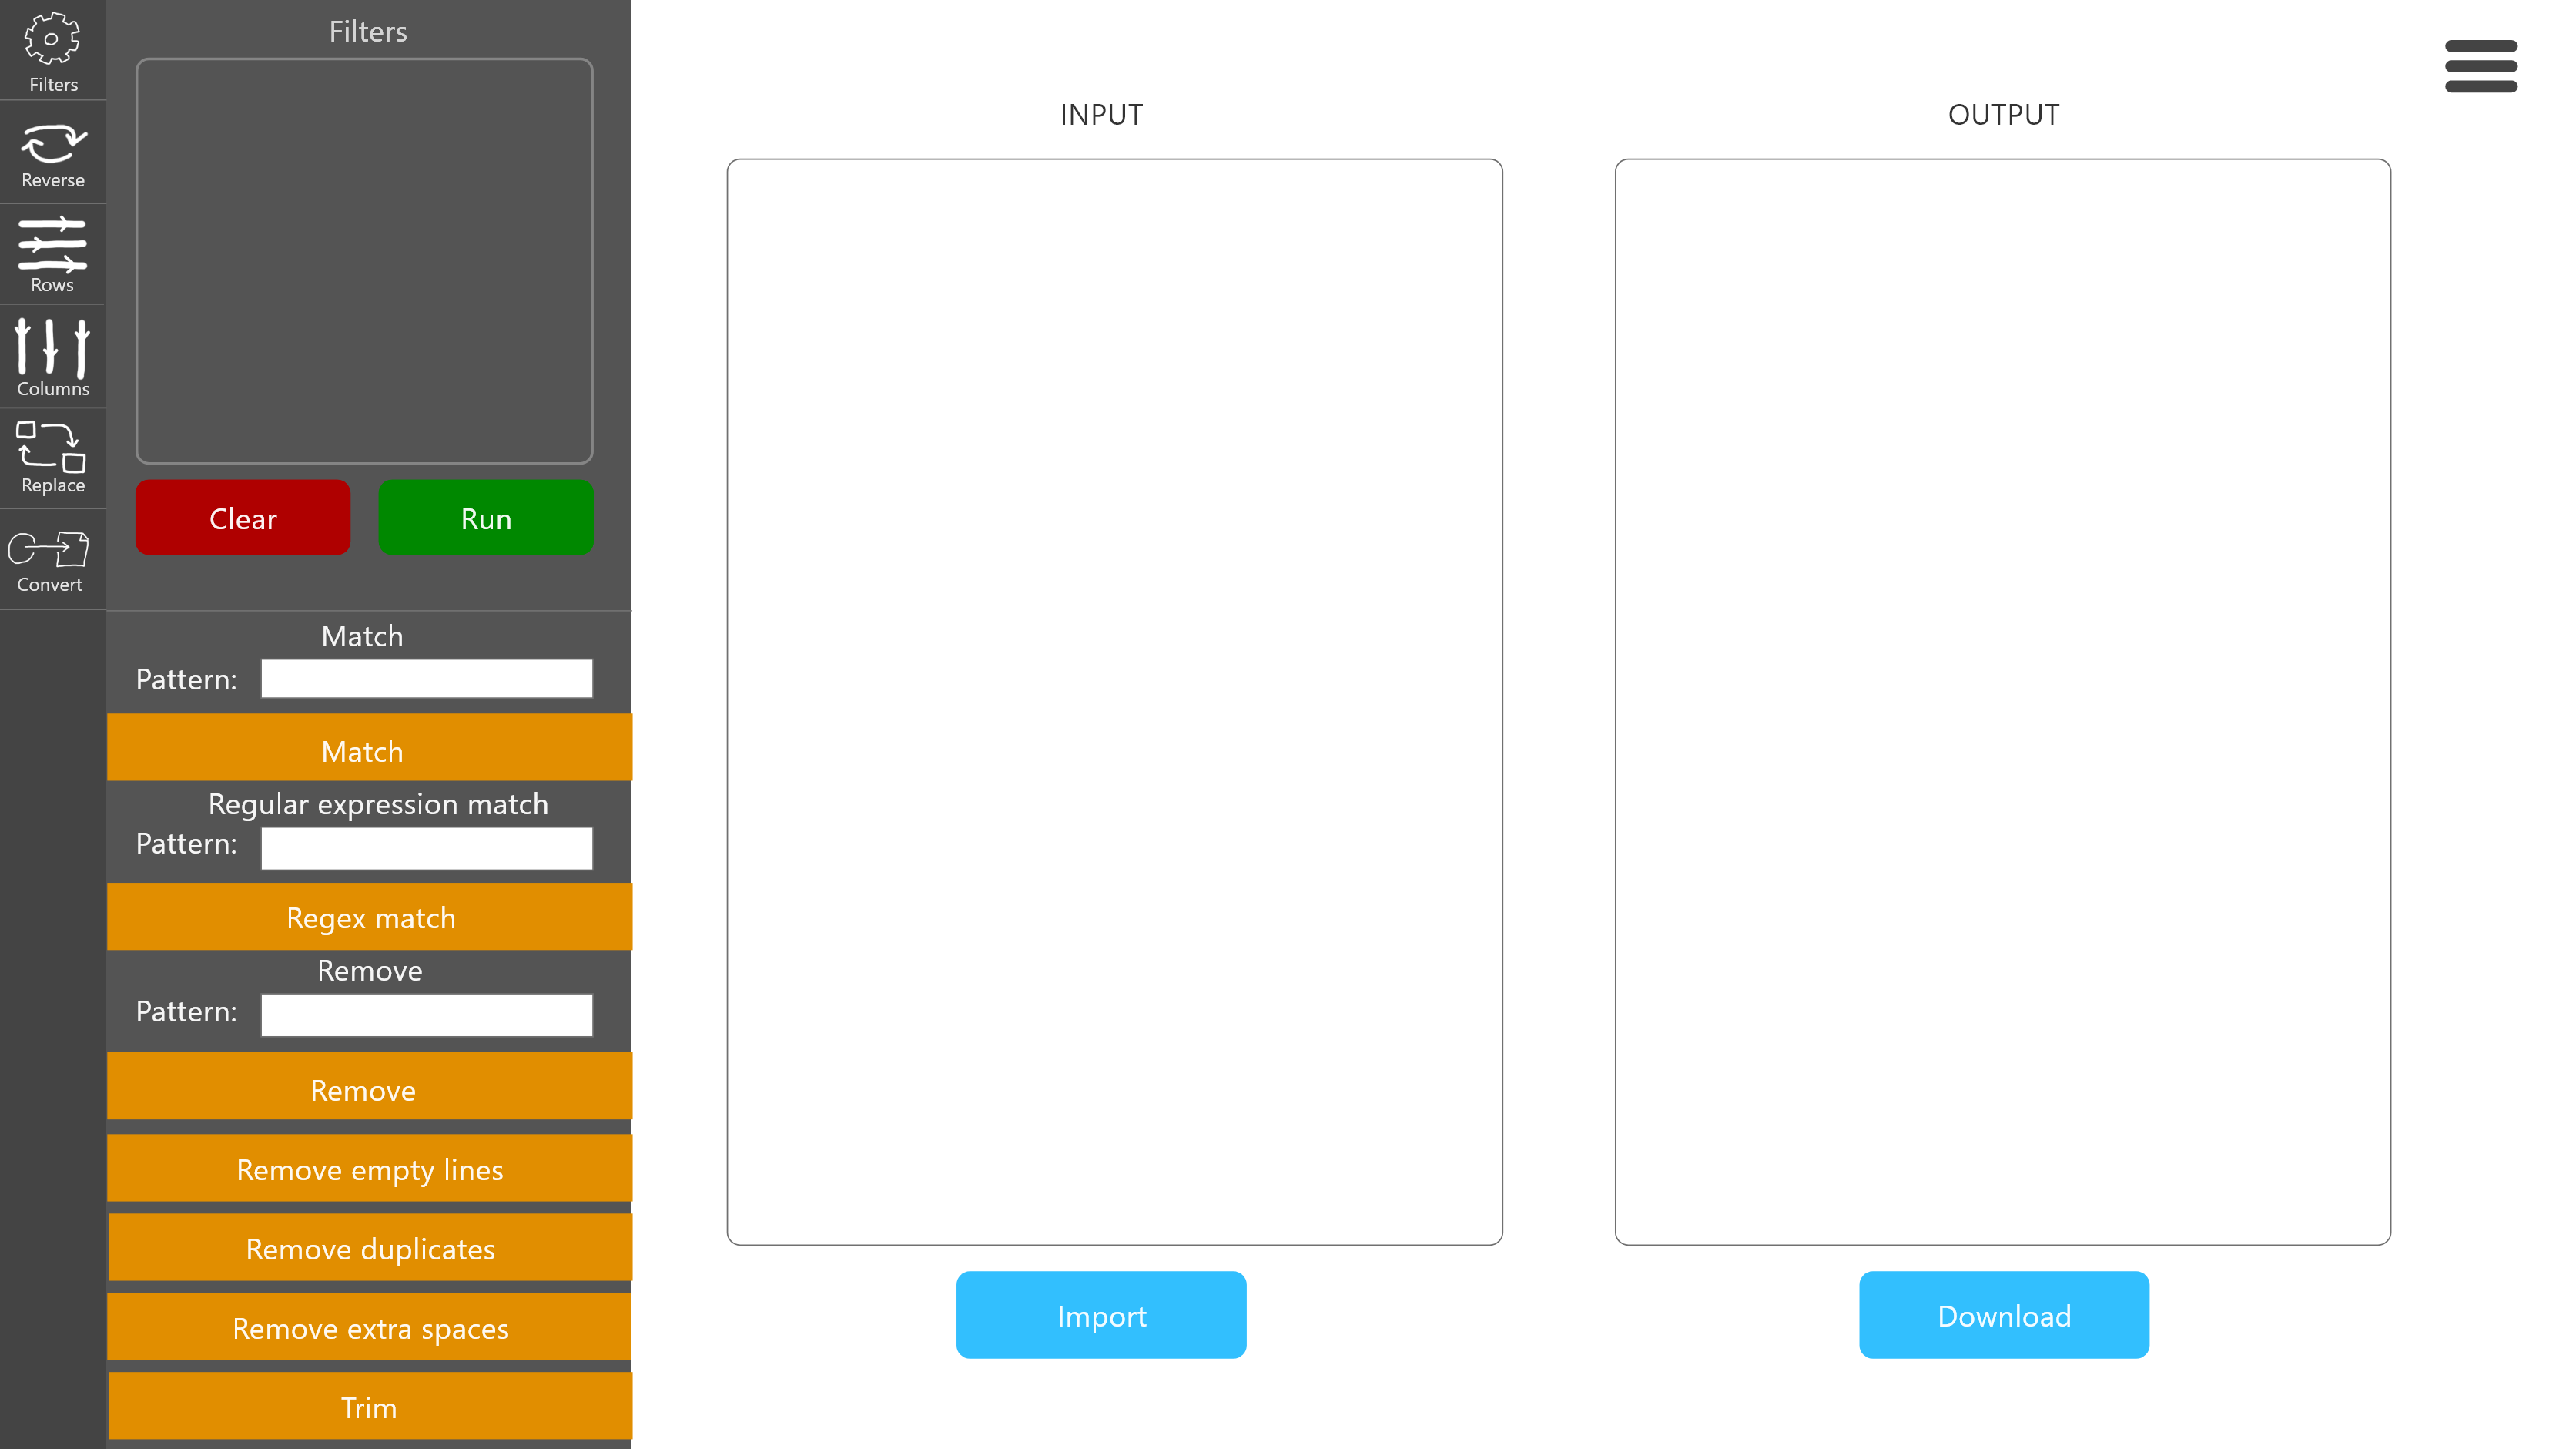
\includegraphics[width=1\textwidth]{obrazky-figures/prvni_navrh.PNG}}
	\caption{První návrh aplikace.}
	\label{obr:První návrh}
\end{figure}

Kategorie nástrojů se nachází vertikálně vlevo a~po jejich volbě by se překreslily pouze nabízené nástroje, přitom horní okénko, které by zobrazovalo seznam použitých nástrojů by zůstalo zobrazené i~nadále a~obsahovalo by pouze názvy. Pod okénkem lze nalézt tlačítka pro spuštění převodu a~odstranění filtrů.

Po předvedení návrhu a~následné konzultaci se ukázalo, že návrh má silné nedostatky už v~základním konceptu. Zejména editory omezují zobrazení textu, lepší by bylo eliminovat všechna prázdná místa okolo, editor maximálně rozšířit a~umožnit uživateli si jeho velikost dynamicky přizpůsobit. Tím se dostáváme k~problému s~nástroji. Vstupy by měly být také širší, protože je vhodné u~dlouhých textů mít možnost se snadno podívat na začátek a~neřešit tento problém posuvníky. Špatné řešení poskytuje také seznam použitých filtrů, jelikož informace pouze o~názvech je nedostačující, matoucí a~při použití více nástrojů stejného typu není jasné, který provádí operaci v~dané konfiguraci. Zároveň převod by se měl provádět automaticky a~nenutit uživatele pokaždé dělat tento úkon manuálně. Tento návrh také neřeší možnost ladění, proto byl vytvořen nový návrh, který je zobrazen na obrázku~\ref{obr:Vylepšený návrh}.
\begin{figure}[H]
	\centering
	\setlength{\fboxsep}{0pt}
	\fbox{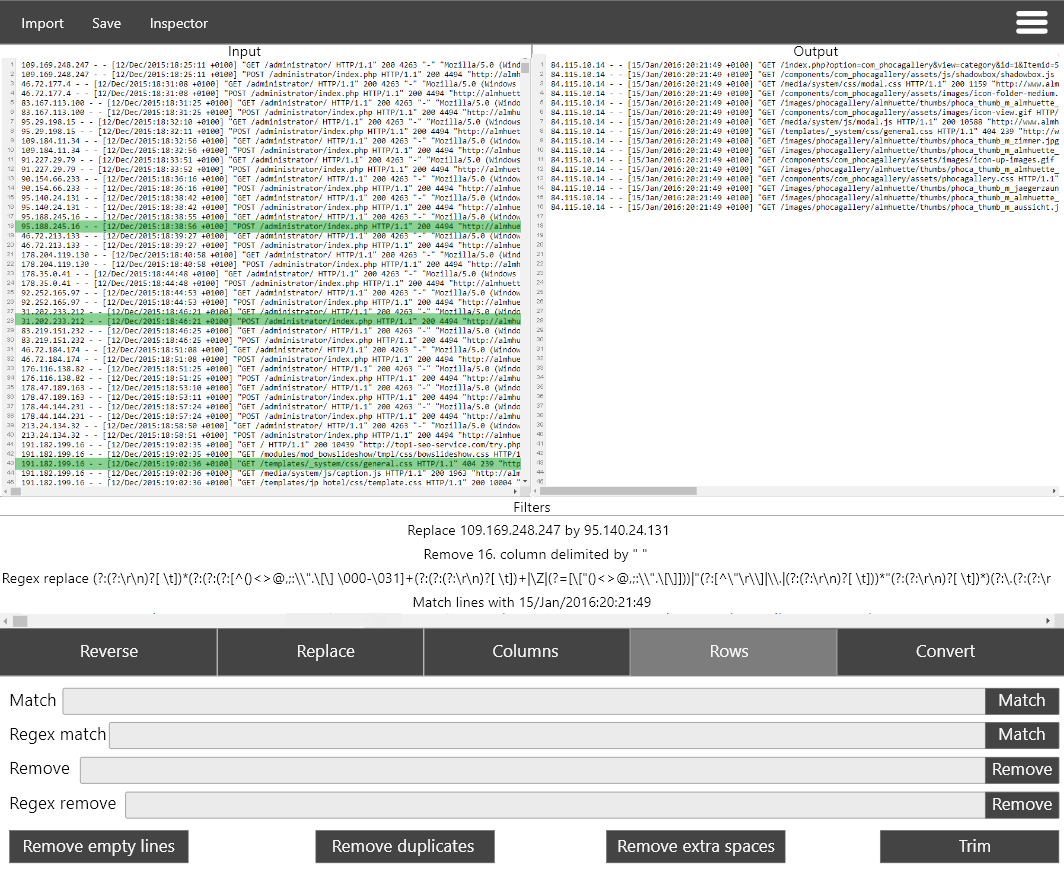
\includegraphics[width=1\textwidth]{obrazky-figures/druhy_navrh.PNG}}
	\caption{Vylepšený návrh aplikace.}
	\label{obr:Vylepšený návrh}
\end{figure}

V novém návrhu byla galerie nástrojů přesunuta z~levé části na spodní část. Tím bylo zajištěno více místa pro vstupy a~popisky. Seznam použitých filtrů byl umístěn pod editor a~také zabírá maximální horizontální prostor, tím je umožněno přehledně vypisovat všechny konfigurace. V tuhle chvíli byl navržen i~styl ladění způsobem vyznačení řádků zelenou barvou, jak je znázorněno na obrázku~\ref{obr:Vylepšený návrh}. Přepínání mezi vyznačováním a~klasickou editací by zajišťovalo tlačítko \uv{inspektor} v~horní liště. Tento návrh poskytl solidní základ pro implementaci a~další vylepšení bylo realizováno na základě testování a~nově vzniklých situací při vývoji celé aplikace.

\subsection*{AdobeXD}
AdobeXD\footnote{AdobeXD: \url{https://www.adobe.com/cz/products/xd.html}}~\cite{article:AdobeXD} je první nástroj od společnosti Adobe navržený přímo pro vývojáře uživatelských rozhraní (dále jen UI). Využívá zkušeností UI návrhářů, kteří používali nástroje jako Photoshop nebo Illustrator a~distribuuje je do jednoho produktu, jehož cílem je zvýšit jejich efektivitu při návrhu.

Designéři v~tomto nástroji mohou snadno přepínat mezi návrhem a~výsledným prototypem (viz obrázek~\ref{obr:Prototyp v AdobeXD}). Veškeré změny v~návrhovém režimu jsou tak hned dostupné v~prototypovacím režimu, což usnadňuje definování aktivních bodů a~přechodů, které oživují maketu. Prototyp aplikace je možné snadno sdílet přes vygenerovaný odkaz a~kdokoliv se na něj může podívat přes webový prohlížeč. Tím je umožněno snadné testování na různých typech zařízení jako jsou mobily, tablety nebo notebooky. Aplikace je zdarma k~použití se základními fonty, omezením pouze na jeden sdílený prototyp a~omezením cloudového úložiště na 2 GB.
\begin{figure}[hbt]
	\centering
	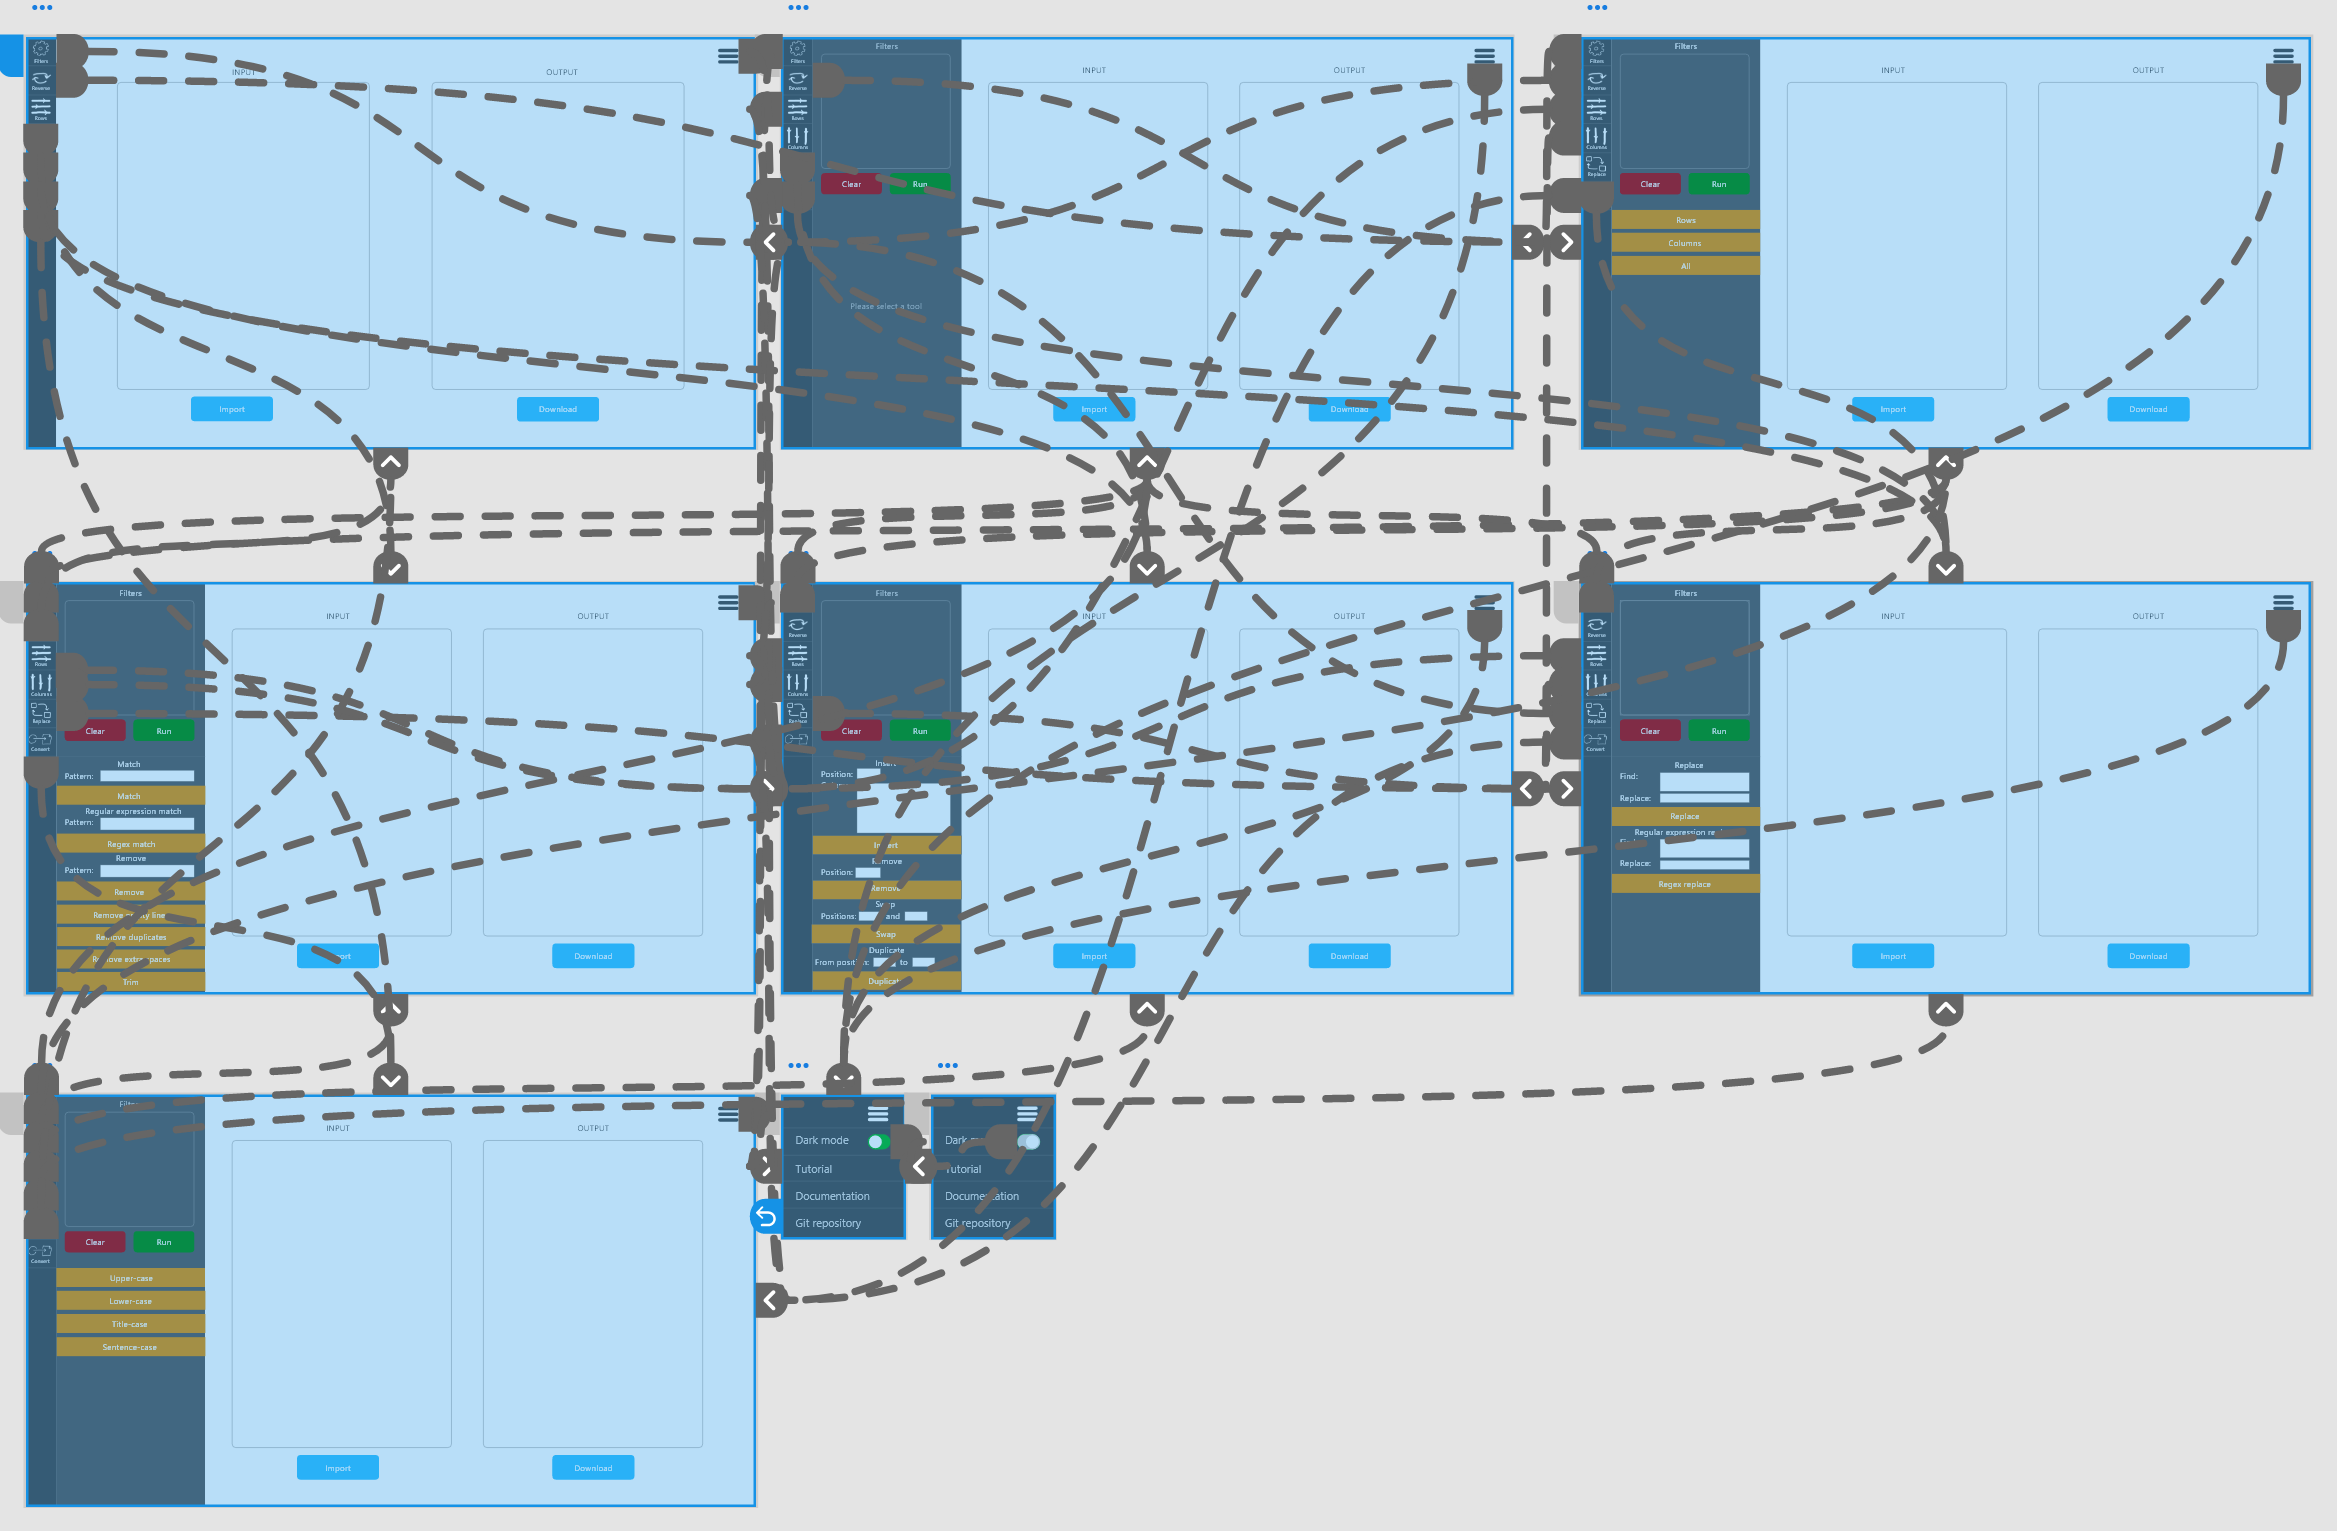
\includegraphics[width=1\textwidth]{obrazky-figures/AdobeXD_prototyp.png}
	\caption{Prototyp aplikace v~AdobeXD.}
	\label{obr:Prototyp v AdobeXD}
\end{figure}

\section{Výběr nástrojů}
Tato činnost byla součástí více etap vývoje. Rozhodování o~tom, zda takový či jiný nástroj by měl být součástí aplikace není záležitostí časově řádu jednotek minut. Jedním z~hlavních specifik a~odlišností této aplikace je skutečnost, že nástroje lze postupně skládat, doplňovat navzájem, a~tak by měly všechny funkce držet tento koncept. Proto mezi opakované typy otázek při výběru patří zejména:
\begin{itemize}
    \item \textbf{Možnost řazení} -- Použití nástroje na text v~originální podobě by mělo umožnit i~další zpracování.
    \item \textbf{Využitelnost} -- Nástroj by neměl být příliš specifický vůči jakémukoliv oboru nebo profesi a~měl by se držet prostého textu.
    \item \textbf{Skriptovací využití} -- Nástroj by měl být vhodně interpretovatelný pro uživatele, kteří využijí vlastnost generování shell skriptů.
    \item \textbf{Zachování kontextu} -- Konzistentní podoba před provedením operace musí zůstat i~po jejím provedení. Jde o~zachování možnosti uživateli poskytnout sledování původního textu.
\end{itemize}

\section{Cílová skupina}
Aplikace je koncipována do široké oblasti využití a~snaží se problematiku spojenou filtrováním snížit na nejnižší možnou úroveň s~cílem oslovit co největší množství potenciálních uživatelů. Zejména se může jednat o~následující:
\begin{itemize}
    \item \textbf{Studenti} -- Často se setkávají s~tabulkovými daty v~projektech nebo při výpisech organizace.
    \item \textbf{Programátoři} -- Úprava dat pro vstupy programů, analýza výstupu. Nejvíce asi ocení možnost generování kódu.
    \item \textbf{Administrativní profese} -- Může se jednat o~profese z~ekonomické sféry nebo publikační agendy.
    \item \textbf{Vědečtí pracovníci} -- Při zpracovávání vědeckých prací či ediční činnosti.
    \item \textbf{Ostatní uživatelé} -- Nejsou příliš nuceni se setkávat s~informacemi v~této podobě a~jde spíše o~jednorázové využití.
\end{itemize}

%=========================================================================
\chapter{Použité technologie}
\label{chap:Použité technologie}

S rostoucí popularitou aplikací vzniklo velké množství balíčků (frameworků), které usnadňují programátorům práci při vývoji. Lze tak vytvářet nové aplikace podstatně rychleji, a~proto nepoužít žádné dostupné řešení v~projektu je dnes velmi neefektivní. V této kapitole budou představeny technologie použité při implementaci a~popsán jejich účel, co nabízí a~jak se s~nimi pracuje. Také budou zmíněny alternativy dostupné na trhu a~důvod, proč byla pro implementaci zvolena právě tato technologie.

\section{Node.js}
Node.js\footnote{Node.js: \url{https://nodejs.org/en}}~\cite{website:GuideToNpm} je open-source prostředí, které umožňuje psát aplikace na straně serveru v~JavaScriptu a~je postavené na JavaScriptovém enginu V8 od Googlu napsaném v~C++. Přesto, že toto rozhraní bylo primárně vytvořeno pro serverové prostředí, používali ho vývojáři při vytváření nástrojů, které jim usnadňovalo práci při jejich úkonech. Od té doby se vyvinul zcela nový ekosystém nástrojů, který změnil způsob vývoje aplikací. Při implementaci byl z~tohoto ekosystému použit nástroj pro správu balíčků, na který se následně zaměříme.

\subsection*{Node Package Manager}
\label{sec:NPM}
Node Package Manager\footnote{NPM: \url{https://www.npmjs.com}} (dále jen NPM) je open-source správce balíčků z~prostředí Node.js. Nenabízí ovšem jen práci s~balíčky, ale zahrnuje kompletní správu projektu od založení projektu až po jeho nasazení na web. Zejména se může jednat o~překlad, sledování závislostí nainstalovaných balíčků a~zranitelností aplikace, definování vlastních skriptů nebo ovládání lokálního serveru.

K vytvoření React webové aplikace (více o~Reactu v~následující kapitole~\ref{sec:React})~\cite{website:createReactApp} je potřeba Node.js verze~8.10 a~vyšší a~NPM verze~5.6 a~vyšší. Samotné vytvoření se provede příkazem \texttt{npx~create-react-app~myApp}, který provede vytvoření celého projektu a~konfiguraci s~tím spojenou. Znamená to, že veškeré nastavování je pro nás jako uživatele už vyřešené a~lze se pustit do implementace. Ovšem v~pozadí se toho děje mnohem více.

Jako první se začne tvořit soubor \texttt{package.json}~\cite{website:WhatDoesCreate-React-AppActuallyDo}, který obsahuje informace o~použitých balíčcích (verze apod.), poté se provede samotná instalace. Jelikož aplikace zatím obsahuje pouze samotný React, nainstaluje pouze jeho knihovny jako React, React-dom a~React-scripts. Po úspěšné instalaci se přesuneme k~nainstalovaným skriptům, které jsou:
\begin{itemize}
    \item \textbf{start} -- Spustí lokální server.
    \item \textbf{build} -- Spustí překlad optimalizovaného kódu aplikace.
    \item \textbf{test} -- Spustí testy.
    \item \textbf{eject} -- Zpřístupní konfiguraci Reactu (jako je Babel, Webpack, ESLint atd.) v~konfiguraci projektu. Vše co je provedeno v~pozadí a~typicky není potřeba dodatečně upravovat manuálně, ale mohou nastat situace, zejména ve větších projektech, kdy se tato vlastnost hodí.
\end{itemize}

Po úspěšné instalaci a~konfiguraci se vytvoří struktura projektu, která je podrobněji popsána v~kapitole~\ref{sec:Struktura projektu}.

\subsection*{Alternativy}
Mezi alternativy je vhodné zmínit open-source nástroj Yarn\footnote{Yarn: \url{https://yarnpkg.com}} vyvinutý společností Facebook. Oproti NPM je rychlejší a~nabízí lepší řešení v~oblasti zabezpečení, kdy v~konfliktu dvou a~více balíčků vznikají chyby v~kódu. To byl také hlavní důvod vzniku tohoto nástroje.

\section{React}
\label{sec:React}
Známé také jako ReactJS\footnote{React: \url{https://reactjs.org}}~\cite{website:EverythingReact} je open-source knihovna pro vytváření uživatelských rozhraní. Nejčastěji se používá při vývoji jednostránkových aplikací tzv.~SPAs (Single Page Applications) a~mobilních aplikací. Je optimalizována pro práci s~rychle se měnícími daty a~překreslováním. Nyní je spravována Facebookem a~komunitou jednotlivých vývojářů a~společností.

Velkou výhodou Reactu je možnost definovat části uživatelského rozhraní na menší celky (komponenty), ty hierarchicky skládat a~znovu používat na více místech. Výsledek z~určité úrovně granularity by pak mohl například vypadat jak na obrázku~\ref{obr:Dekompozice rozhraní na menší komponenty}.
\begin{figure}[hbt]
	\centering
	\setlength{\fboxsep}{0pt}
	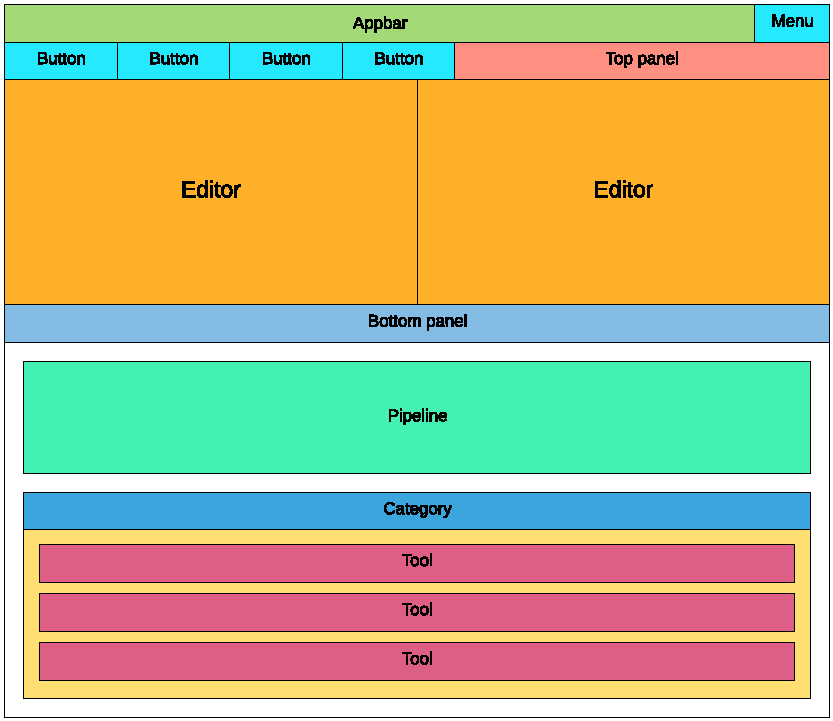
\includegraphics[width=0.8\textwidth]{obrazky-figures/dekompozice_rozhrani.pdf}
	\caption{Dekompozice rozhraní aplikace na menší komponenty.}
	\label{obr:Dekompozice rozhraní na menší komponenty}
\end{figure}

React je poměrně velká a~komplexní knihovna, která nabízí nejen kvalitní řešení, ale poskytuje i~větší pohodlí při vývoji. K~zajištění takové funkcionality musí spolupracovat se spoustou dalších metod a~balíčků. Mezi ty nejdůležitější patří:
\begin{itemize}
    \item \textbf{JSX} -- Syntax připomíná HTML, ale ve skutečnosti jde o~rozšíření pro JavaScript k~definování React prvků. Samotný React ho ovšem nevyžaduje, ale je velmi nápomocný.
    \lstdefinelanguage{jsx}{
        morekeywords={
            const,
            <h1>,
            </h1>
        },
        sensitive=false,
        morestring=[b]"
    }
    \lstset{
        language={jsx},
        keywordstyle=\color{blue},
    }
    \begin{center}
        \begin{lstlisting}[]
        const element = <h1>Hello, world!</h1>;
        \end{lstlisting}
    \end{center}

    \item \textbf{Babel\footnote{Babel: \url{https://babeljs.io}}} -- Protože React aplikace je napsána v~JSX a~webové prohlížeče této syntaxi nerozumí, vzniká problém. Tady přichází do hry Babel. Je to open-source JavaScriptový kompilátor, který převádí JSX zápis na prostý JavaScript.
    \item \textbf{Webpack\footnote{Webpack: \url{https://webpack.js.org}}} -- Je nástroj~\cite{book:LearningReact} pro zpracování souborů a~usnadnění práce vývojářů. Jeho primárním účelem je vytvořit balíčky z~modulárního JavaScriptového kódu pro jeho použití v~prohlížeči. Neomezuje se ovšem pouze na JavaScriptové soubory, ale umožňuje zpracovat téměř jakýkoliv druh jako jsou obrázky, serializační formáty aj. Výstupem je modulární JavaScriptový balíček.
\end{itemize}

Další balíčky, se kterými může React pracovat, jsou znázorněny na obrázku~\ref{obr:Ekosystém Reactu}. Ve skutečnosti se všemi najednou nepracuje, záleží především na požadavku výsledné aplikace.
\begin{figure}[hbt]
	\centering
	\setlength{\fboxsep}{0pt}
	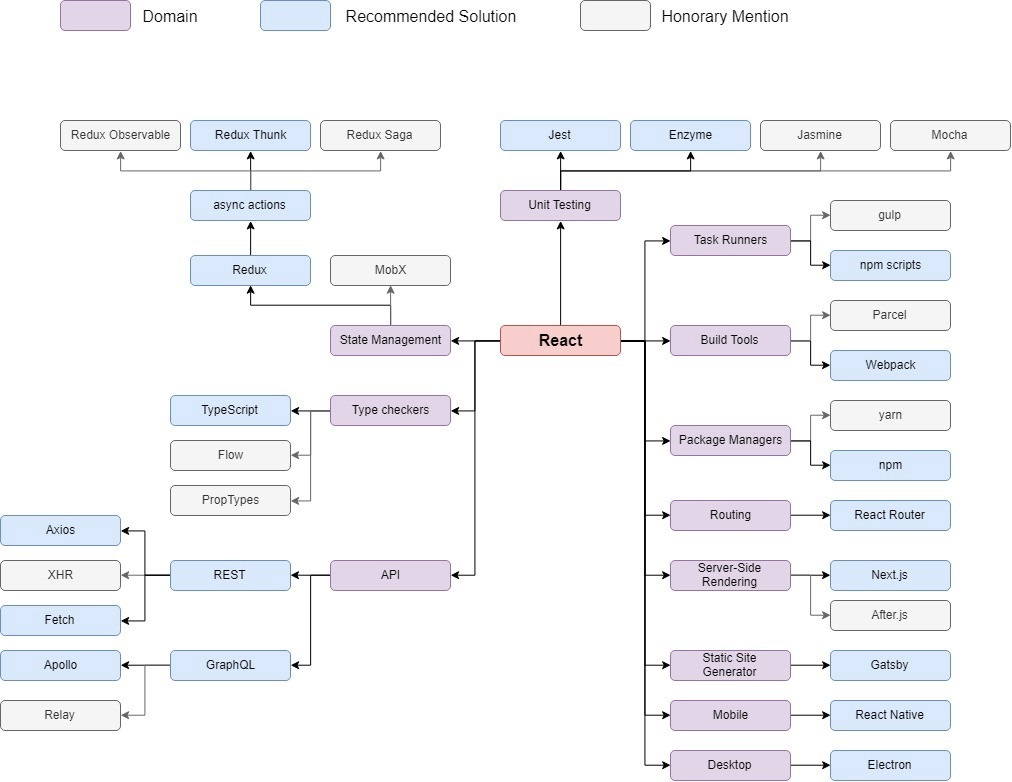
\includegraphics[width=1\textwidth]{obrazky-figures/ReactEcosystem.png}
	\caption{Podmnožina ekosystému Reactu. Zde jsou znázorněny některé známé, často používané balíčky. Výsledný ekosystém je znatelně větší. Převzato z~\cite{website:EverythingReact}.}
	\label{obr:Ekosystém Reactu}
\end{figure}

\subsection*{Vznik a historie}
ReactJS~\cite{website:ReactHistory} začal jako JavaScriptový port XPH od Facebooku při řešení problému s~minimalizací útoku cross-site scripting (XSS). Tento typ útoku spočívá ve využití chyb ve skriptech běžících na webu (především neošetřené vstupy). Útočník může takto do stránek podstrčit vlastní JavaScriptový kód, který dokáže poškodit vzhled stránky, znefunkčnit ji nebo získat citlivé údaje návštěvníků. Tato metoda je též často využívána při phishingu. Nastal však problém, kdy dynamické webové stránky poskytují dlouhou zpáteční cestu na server a~XHP tento problém nevyřeší. Došlo tak k~zavedení XHP do prohlížeče pomocí JavaScripu. Výsledkem byl React.

\subsection*{Objektový model dokumentu}
Objektový model dokumentu~\cite{article:BeginnersGuideToReact} (dále jen DOM) z~anglického názvu Document Object Model je multiplatformní a~jazykově nezávislé rozhraní reprezentující HTML, XHTML nebo XML jako logickou stromovou strukturu.

React~\cite{book:LearningReact, article:BeginnersGuideToReact} vytváří v~mezipaměti strukturu zvanou \textbf{Virtuální DOM}, ve které vypočítává provedené změny a~poté aktualizuje DOM prohlížeče. Tato vlastnost umožňuje programátorům naprogramovat celou aplikaci se závislostmi, při kterých je potřeba překreslení. Knihovna poté bude tyto části aplikace překreslovat pouze, pokud je doopravdy provedena změna, a~je tak umožněno aktualizovat pouze jeden DOM element, který se změnil. React provádí proces aktualizace ve třech krocích:
\begin{enumerate}
    \item Po změně prvku se překreslí celý virtuální DOM Reactu.
    \item Provede se porovnání s~předchozí DOM reprezentací.
    \item Skutečný DOM prohlížeče bude aktualizován na základě změn porovnání. Tento krok může připomínat použití opravného patche (viz obrázek~\ref{obr:Porovnani DOMu}).
\end{enumerate}

\begin{figure}[hbt]
	\centering
	\setlength{\fboxsep}{0pt}
	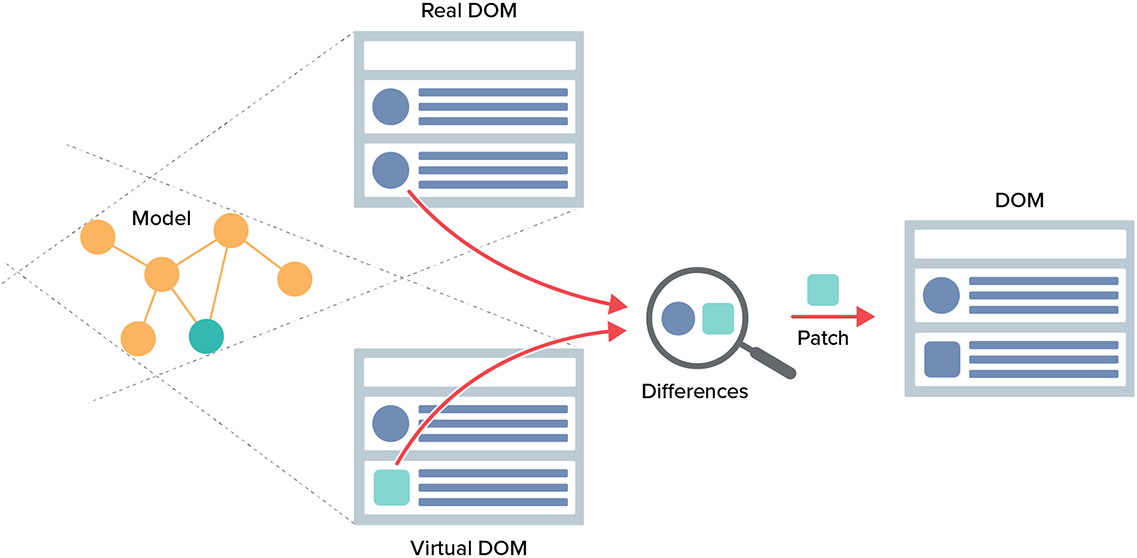
\includegraphics[width=1\textwidth]{obrazky-figures/porovnani_DOMu.png}
	\caption{Proces aktualizace struktury DOM v~Reactu. Převzato z~\cite{article:BeginnersGuideToReact}.}
	\label{obr:Porovnani DOMu}
\end{figure}

\subsection*{Komponenty}
\label{sec:Komponenty}
Komponenty~\cite{article:BeginnersGuideToReact} jsou modulární části kódu, které umožňují rozdělit uživatelské rozhraní na nezávislé, opakovaně použitelné kusy. Koncepčně jsou komponenty jako JavaScriptové funkce, které přijímají libovolné vstupy (props) a~vracejí prvky Reactu, které popisují výslednou podobu na obrazovce. Mezi dobré zásady patří skládání komponent do logické stromové struktury předávající si parametry z nadřazené komponenty k~podřízené, tedy směrem shora dolů tak, jak je znázorněno na obrázku~\ref{obr:Hierarchie komponent}. Pokud nadřazená komponenta bere vstup z~podřízené přes referenci, typicky tato situace indikuje, že je dostupné lepší řešení. Ovšem existují situace, kdy takové řešení je nejlepší, například u~přehrávání animací nebo při použití externích knihoven.

Chování aplikace neboli komponenty v~daném okamžiku je definováno jejím aktuálním stavem. Stav obsahuje data, která se mění na základě interakce s~uživatelem, obvykle obsluhou událostí. Jinak řečeno, když se změní stav komponenty, React znovu vykreslí odpovídající část do prohlížeče. Vstupy komponenty jsou na rozdíl od stavu neměnné a~nastavují se nadřazenou komponentou. Komponenty můžeme rozdělit podle stavu na:
\begin{itemize}
    \item \textbf{Bezstavové}
        \begin{itemize}
            \item Nemají žádný stav
            \item Mají vstupy
            \item Překreslení je závislé na vstupech
        \end{itemize}
    \item \textbf{Stavové}
        \begin{itemize}
            \item Mají měnící se stav
            \item Stav nelze číst a~nastavit mimo komponentu
            \item Mají vstupy
            \item Překreslení je závislé na vstupech a~stavu
        \end{itemize}
\end{itemize}

\begin{figure}[hbt]
	\centering
	\setlength{\fboxsep}{0pt}
	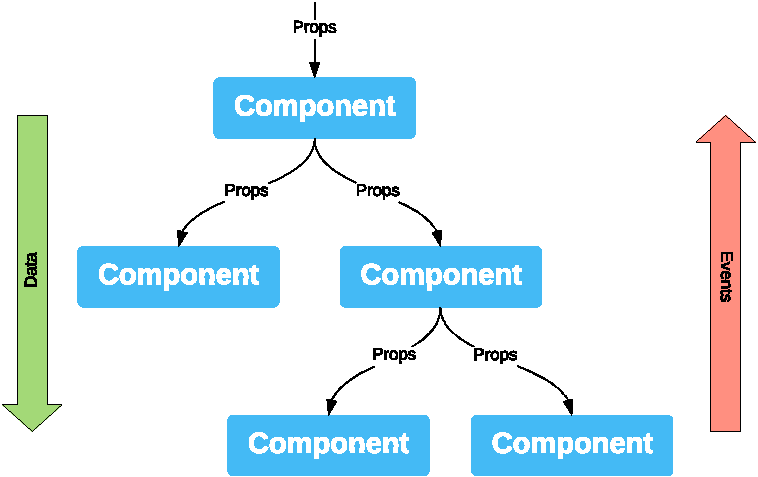
\includegraphics[width=0.75\textwidth]{obrazky-figures/hierarchie_komponent.pdf}
	\caption{Hierarchie React komponent ve stromové struktuře.}
	\label{obr:Hierarchie komponent}
\end{figure}

Samotné komponenty lze implementovat ve dvou zápisech, a~to třídním nebo funkcionálním a~je vhodné se tohoto zápisu držet v~celém projektu. Nejviditelnějším rozdílem je syntax a~také, že Babel v~případě třídní komponenty transponuje více kódu. Funkcionální komponenty jsou snadněji čitelné než třídní, protože připomínají spíše funkce. Od verze~16.8 disponují funkcionální komponenty také hooky a~jsou tak funkčně ekvivalentní s~těmi třídními. Dříve se používaly pouze u~bezstavových komponent.

\subsection*{Životní cyklus komponent a React hooks}
\label{sec:Životní cyklus komponent a React hooks}
Životní cyklus komponent~\cite{article:BeginnersGuideToReact} je znázorněn na obrázku~\ref{obr:Fáze životního cyklu komponenty} a~probíhá ve třech fázích: montování, aktualizace a~odpojování. V těchto fázích probíhají metody zvané \uv{hooks}, ke kterým dochází v~určitém pořadí jak je znázorněno na obrázku~\ref{obr:Výskyt hooků ve fázích životního cyklu komponenty}.
\begin{figure}[hbt]
	\centering
	\setlength{\fboxsep}{0pt}
	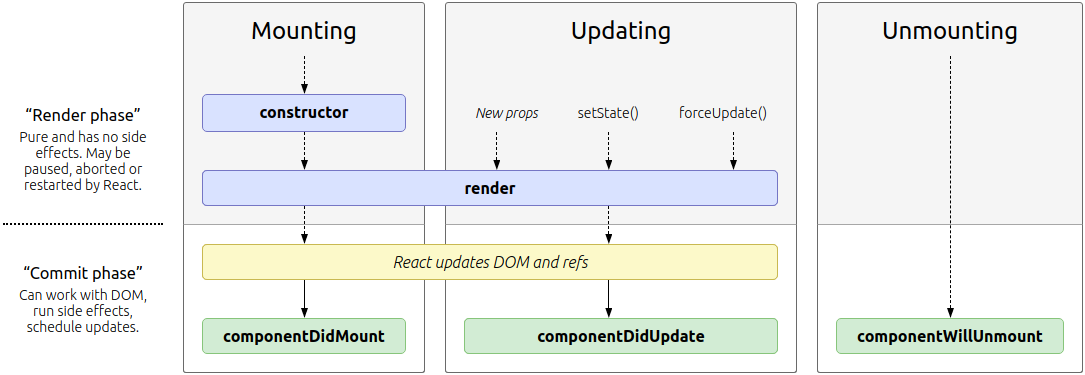
\includegraphics[width=1\textwidth]{obrazky-figures/faze_komponenty.png}
	\caption{Fáze životního cyklu komponenty. Převzato z~\cite{article:BeginnersGuideToReact}.}
	\label{obr:Fáze životního cyklu komponenty}
\end{figure}

\begin{itemize}
    \item \textbf{Montování}
        \begin{enumerate}
            \item \textbf{\texttt{constructor()}} -- Zde lze inicializovat počáteční stav komponenty a~navázat metody pro obsluhu událostí.
            \item \textbf{\texttt{componentWillMount()}} -- Metoda je zavolána před započetím montování.
            \item \textbf{\texttt{render()}} -- První vykreslení, jedná se tedy o~montování komponenty.
            \item \textbf{\texttt{componentDidMount()}} -- Metoda je zavolána po ukončení montování.
        \end{enumerate}
    \clearpage
    \item \textbf{Aktualizace}
        \begin{enumerate}
            \item \textbf{\texttt{componentWillReceiveProps()}} -- Metoda je zavolána u~namontované komponenty před obdržením nových vstupu.
            \item \textbf{\texttt{shouldComponentUpdate()}} -- Ve výchozím režimu React překreslí komponentu kdykoliv se změní stav nebo vstup. Tato metoda oznamuje, že výstup komponenty není závislý na daném typu dat, a~tak není nutné překreslení. Slouží jako optimalizační metoda.
            \item \textbf{\texttt{componentWillUpdate()}} -- Metoda je zavolána vždy před započetím překreslení.
            \item \textbf{\texttt{render()}} -- Překreslení komponenty.
            \item \textbf{\texttt{componentDidUpdate()}} -- Metoda je zavolána okamžitě po překreslení komponenty. Neplatí pro první vykreslení.
        \end{enumerate}
    \item \textbf{Odpojování}
        \begin{enumerate}
            \item \textbf{\texttt{componentWillUnmount()}} -- Metoda je zavolána před odpojením a~zničením komponenty. Běžně se používá pro uvolnění alokovaných zdrojů.
        \end{enumerate}
\end{itemize}
\begin{figure}[hbt]
	\centering
	\setlength{\fboxsep}{0pt}
	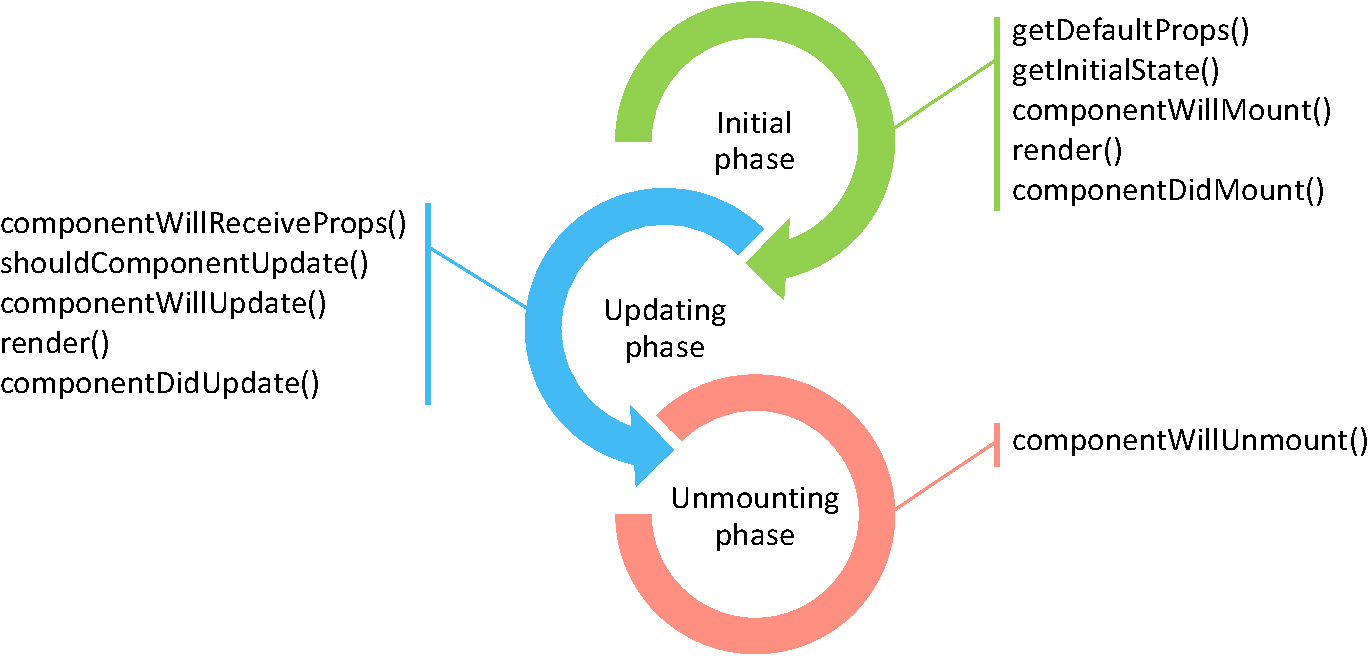
\includegraphics[width=1\textwidth]{obrazky-figures/hooky_ve_fazich.pdf}
	\caption{Výskyt hooků ve fázích životního cyklu komponenty. Inspirováno z~\cite{article:BeginnersGuideToReact}.}
	\label{obr:Výskyt hooků ve fázích životního cyklu komponenty}
\end{figure}

V případě funkcionálních komponent se využívají jiné hooky, které nabízí podobnou funkcionalitu jako předchozí zmíněné. Jelikož aplikace je implementována ve funkcionálním zápisu, tak zde jsou uvedeny alespoň ty nejpodstatnější:
\begin{itemize}
    \item \textbf{\texttt{useState()}} -- Slouží k~definici stavu komponenty. Jelikož se jedná o~funkce, je nutno explicitně říct Reactu, na základě kterých stavů má být provedeno překreslení.
    \item \textbf{\texttt{useEffect()}} -- Tento hook je zavolán vždy po změně stavu komponenty s~možností definovat stavy, které mají být sledovány. Pokud není definováno, chová se jako metoda \texttt{componentDidUpdate()}. Nabízí také tzv.~\uv{clean-up effect} neboli vyčištění, ve kterém lze po provedení metody uvolnit alokované zdroje. V takové kombinaci lze dosáhnout i~chování \texttt{componentDidMoount()} nebo \texttt{componentWillUnmount()}.
    \item \textbf{\texttt{useCallback()}} -- Optimalizační metoda. Slouží pro definování stavů, které ovlivní přetvoření funkce. Ve výchozím režimu, vždy po překreslení komponenty se přetvoří i~funkce, které obsahuje, i~když se jejich kód nezměnil, to pak způsobí překreslení všech následujících komponent, které přijímají tuhle funkci jako vstup.
    \item \textbf{\texttt{useRef()}} -- Umožňuje odkazovat podřízenou komponentu a~přistoupit tak k~jejím instancím.
    \item \textbf{\texttt{useImperativeHandle()}} -- Definuje instance, které budou zpřístupněny nadřazené komponentě. Takto nadřazená komponenta pak může k~těmto instancím přistoupit přes referenci.
    \item \textbf{\texttt{useMemo()}} -- Slouží k~memorování předchozího průběhu. Typicky se tato metoda využívá na místech, kde je kód často prováděný (např. funkce) k~urychlení výpočtu. Není vhodné tuto metodu používat všude, ale jen na určitých místech, kde dochází k~viditelnému zpomalení.
\end{itemize}

\subsection*{Shrnutí a alternativy}
React je v~současnosti nejpopulárnější knihovna svého druhu, která nabízí spoustu možností a~stále se rozrůstá. Používají ji velké společnosti jako Facebook, Instagram nebo Netflix. Nabízí velkou rychlost zpracování díky implementaci virtuální struktury DOM. Další podstatnou výhodou je, že volba konceptu programování je ponechána na uživateli mezi funkcionálním a~třídně založeným stylem. Oproti tomu jsou zde i~nevýhody jako je dělení kaskádových stylů do zvláštních souborů nebo zavedení přímo do komponent a~míchání logiky programu se šablonami, což může být pro některé uživatele matoucí.

Alternativou může být knihovna \textbf{Angular\footnote{Angular: \url{https://angular.io}}} od společnosti Google, kterou využívají například společnosti Microsoft, Apple a~AT\&T. Angular~\cite{website:AngularVsReactVsVue} přebírá mnoho konceptů z~návrhového vzoru Model-View-ViewModel (MVVM), který umožňuje přehledně oddělit logiku od rozhraní aplikace a~má mimořádnou podporu TypeScriptu. Struktura a~architektura je navržena speciálně  pro velkou škálovatelnost projektu. Mezi nevýhody patří poměrně malý výkon a~poměrně vysoká složitost.

Další v~dnešní době velmi známou alternativou je knihovna \textbf{VueJS\footnote{VueJS: \url{https://vuejs.org}}}, za kterou nestojí žádná velká společnost a~využívají ji společnosti jako GitLab, Adobe a~Xiaomi. Knihovna~\cite{website:AngularVsReactVsVue} nabízí detailní dokumentaci a~umožňuje vytvářet znovupoužitelné šablony. V mnoha ohledech si bere inspiraci z~Reactu a~Angularu, to umožňuje snadnější přestup mezi knihovnami. Mezi nevýhody patří nedostatečná podpora integrace do větších projektů a~menší ekosystém oproti dříve zmíněným knihovnám.

\section{Material-UI}
Material-UI\footnote{Material-UI: \url{https://material-ui.com}} je dnes jeden z~oblíbených React frameworků pro tvorbu uživatelských rozhraní, který vznikl v~roce 2014 na implementaci material designu\footnote{Material design: \url{https://material.io}}. Mezi společnosti využívající Material-UI patří např. Bethesda, Amazon a~Unity. Framework nabízí předdefinované části rozhraní (elementy) jako React komponenty s~cílem usnadnit a~zrychlit tvorbu a~zároveň zajistit vyšší míru kvality. V současné verzi 4.9.8 má Material-UI přes 5 milionů stažení měsíčně přes správce balíčku NPM (viz kapitola~\ref{sec:NPM}).

Material-UI poskytuje také balíček s~ikonami, který lze dodatečně přidat. Sada nabízí přes $1\,100$~ikon, které jsou ve většině případů zaměřené spíše na mobilní zařízení, přesto v~tomhle projektu je sada postačující, a~tak není nutné importovat další. Způsob zacházení je potom stejný jako s~ostatními prvky Material-UI nebo komponenty.

\subsection*{Material design}
Jde v~zásadě o~filozofii designu (tzv.~vizuální jazyk), kterou Google~\cite{book:MaterialDesign} poprvé představil v~roce 2014 na konferenci Google I/O. Primárně je určen pro mobilní platformu, ale principy se přenesly napříč všemi zařízeními. Material design poskytuje návod na podobu rozhraní od rozvržení přes animace až po barvy. Samotný koncept je inspirován reálným světem a~jeho texturami, včetně toho, jak se odráží světlo a~vznikají stíny na povrchu materiálů, odtud byl přejat název \uv{material}.

\subsection*{Alternativy}
Známou alternativou a~jednou z~nejstarších je knihovna Bootstrap, přesněji pro React knihovna React-Bootstrap\footnote{React-Bootstrap: \url{https://react-bootstrap.github.io}}, která poskytuje prvky jako React komponenty bez dodatečných závislostí (třeba na jQuery). Výhodou je soulad mezi prohlížeči, takže by se stránka měla vždy korektně vykreslovat a~zároveň není náročná. Mezi nevýhody patří špatná přizpůsobitelnost, což může vést k~podobám mezi weby, které spolu ani nemusí souviset.

\section{Ace editor}
Jak je zmíněno v~kapitole~\ref{sec:Požadavky na webovou aplikaci}, editor je základ celé aplikace, a~proto by měl nabízet také mnoho funkcí. S~takovými je možné se setkat například v~programování. Editor, který poskytne programátorovi největší komfort se stane velmi oblíbený. Tady se naskytuje možnost tento editor využít a~předělat ho na potřeby této aplikace.

Jedním z~těchto editorů je open-source Ace\footnote{Ace editor: \url{https://ace.c9.io}} poskytovaný s~BSD licencí, jedná se tedy o~svobodný software s~volným šířením. Ace je napsán v~JavaScriptu a~udržován jako primární editor pro Cloud9 IDE\footnote{Cloud9 IDE: \url{https://aws.amazon.com/cloud9}} a~je nástupcem projektu Mozilla Skywriter\footnote{Mozilla Skywriter: \url{https://www.mozillalabs.com/en-US/skywriter/index.html}} (dříve Bespin). Nyní je Ace jedním z~nejpopulárnějších webových editorů vůbec a~je používán v~projektech jako Codebender, Overleaf nebo Wikipedia.

Samotný Ace nabízí vysoký výkon pro editaci textu, oficiální stránka udává limit na 4~milióny řádků, ale záleží na průměrném počtu znaků na řádek. Dále je možné využít zvýrazňování syntaxe, přes 20~motivů, číslování řádků, klávesové zkratky a~další. Nejzajímavější vlastností je ovšem ladící rozhraní určené pro programátory, které bylo přizpůsobeno na potřeby této aplikace. Při implementaci byl použit oficiální wrapper\footnote{Ace wrapper: \url{https://github.com/securingsincity/react-ace}} pro React, který zpřístupňuje Ace jako komponentu. Další práce je tak umožněna přes vstupy nebo referenci. V opačném případě by bylo potřeba vytvořit vlastní wrapper.

\subsection*{Alternativy}
Druhý v~dnešním trendu je editor \textbf{CodeMirror\footnote{CodeMirror: \url{https://codemirror.net}}}, který v~aktuální verzi~5.52.2 nabízí přehlednou dokumentaci a~velmi podobnou funkcionalitu jako výše zmíněný Ace. Je používaný v~projektech jako Adobe Brackets, JSFiddle nebo GitHub. Další vhodnou alternativou je \textbf{Monaco\footnote{Monaco: \url{https://microsoft.github.io/monaco-editor}}} vyvinutý společností Microsoft. Editor nabízí moderní vzhled a~mini-mapu celého dokumentu, která usnadňuje orientaci. Mezi nevýhody patří nepodporované mobilní zařízení a~poměrně malá sada poskytnutých nástrojů oproti výše zmíněným editorům. Projekty, které využívají Monaco jsou např. Visual Studio Code nebo CodeSandbox.

\section{Web worker}
Web worker API~\cite{website:WebWorkers} je JavaScriptový kód běžící v~pozadí aplikace, bez narušení výkonu stránky. Obecně JavaScript je jednovláknový a~může provádět jen jednu operaci v~daný okamžik. Zde však vzniká problém s~výpočetně náročnými operacemi nebo operacemi nad obsáhlými daty, protože i~během tohoto výpočtu je potřeba neustále reagovat na události od uživatele, jinak by mohla nastat situace, kdy se uživatel snaží provést úkon ve své úloze, ale aplikace nereaguje, protože počítá výsledek. V tomto případě je zapotřebí zavést pojem vícevláknové zpracování.

API komunikuje s~hlavní aplikací pomocí metody zasílání zpráv. Hlavní aplikace pošle požadavek skriptu a~následně dostává odpovědi. Během procesu zpracování se pak může dále věnovat požadavkům uživatele. V případě této aplikace je řešení této problematiky nutné z~důvodu, že data získána od uživatele mohou být rozsáhlá a~také zpracování textových operací je poměrně náročné, jak bylo již dříve zmíněno v~kapitole~\ref{sec:Informovat uživatele}.

Konkrétně vždy, když je potřeba data zpracovat, odešle hlavní aplikace zprávu s~daty a~informacemi o~způsobu jejich zpracování, ty obsahují například použité nástroje a~jejich konfiguraci, stav editoru aj. Vlákno poté začne data zpracovávat, informuje o~aktuálním stavu procesu převodu hlavní aplikaci a~nakonec ji pošle výsledek. Tím se dostáváme k~zavedení typu zpráv. Během získávání odpovědí do aplikace je potřeba rozlišit, jak interpretovat danou odpověď. Pokud se jedná o~odpověď nesoucí informaci, že proces transformace je například z~$80\%$ kompletní, je tato informace sdělena uživateli, pokud se jedná o odpověď obsahující výsledek převodu, tak je tento výsledek zobrazen. Proto každá zpráva musí obsahovat typ, který identifikuje její obsah. Proces komunikace pak může vypadat jak na obrázku~\ref{obr:Komunikace mezi aplikací a web workerem}.

\begin{figure}[hbt]
	\centering
	\setlength{\fboxsep}{0pt}
	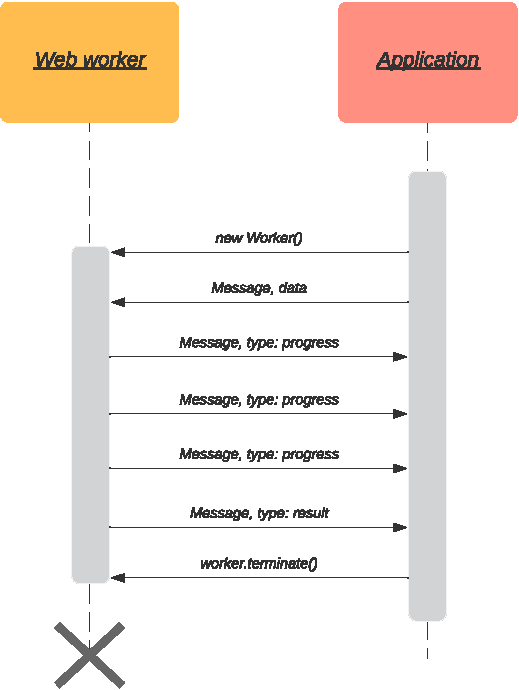
\includegraphics[width=0.6\textwidth]{obrazky-figures/app-worker_komunikace.pdf}
	\caption{Komunikace mezi aplikací a~web workerem.}
	\label{obr:Komunikace mezi aplikací a web workerem}
\end{figure}

\section{Selenium}
\label{sec:Selenium}
Selenium\footnote{Selenium: \url{https://www.selenium.dev}} \cite{website:Selenium} je open-source platformově nezávislý nástroj implementovaný v~Javě pro automatické testování webových aplikací nebo e-shopů v~různých prohlížečích. Samotné testy je možné vytvářet interaktivně pomocí Selenium IDE\footnote{Selenium IDE: \url{https://www.selenium.dev/selenium-ide}} v~prohlížeči nebo pomocí programovacích jazyků jako jsou Java, Python, Perl, PHP nebo Ruby. Selenium může být zároveň integrován nástroji pro správu testů.

\subsection*{Sada nástrojů}
Selenium také poskytuje následující sadu nástrojů, které usnadňují testování:
\begin{itemize}
    \item \textbf{Selenium IDE} -- Je dostupné jako rozšíření do webového prohlížeče Firefox nebo Chrome. Toto prostředí nabízí nejjednodušší způsob pro tvorbu testů jednoduchou uživatelskou interakcí v~prohlížeči a~následným vygenerováním skriptu provádějící tuto sekvenci událostí. Tato metoda nevyžaduje znalost programování.
    \item \textbf{Selenium RC} -- Jedná se o~proxy server pro instance webových prohlížečů, který přijímá příkazy z~podporovaných jazyků uživatelských programů a~předává je do prohlížeče. Po zprovoznění serveru se k~němu klienti připojují a~spouští své testy, jedná se o~klasické klient-server řešení.
    \item \textbf{Selenium WebDriver} -- Umožňuje pracovat lokálně přímo s~aplikacemi prohlížečů. Není proto nutné nastavovat Selenium server, nicméně je nutné nastavit ovladač pro každý prohlížeč zvlášť.
    \item \textbf{Selenium Grid} -- Umožňuje \cite{website:Selenium} spouštět testy paralelně na několika počítačích v~různých prostředích na různých operačních systémech. Jedná se o~rozbočovač připojený k~několika uzlům. Přijatý test je poté předán uzlu, který odpovídá požadavkům (platforma a~prohlížeč), ve kterém má být spuštěn.
\end{itemize}

\section{GitHub Pages}
\label{sec:GitHub Pages}
GitHub Pages\footnote{GitHub Pages: \url{https://pages.github.com}} je webhostingová služba poskytovaná od roku~2008 společností GitHub, u~které byl projekt také verzován během implementace a~následně zveřejněn. Výchozí stránky jsou dostupné pod doménou \texttt{github.io}, ale je možné nastavit i~vlastní. V roce~2016 začaly být stránky poskytovány pod šifrovaným protokolem HTTPS. Tato služba~\cite{website:ghpages} nesmí být ovšem využívána jako bezplatný webhosting k~provozování online obchodu, komerčních webů nebo jiných webů, které jsou primárně určeny k~obchodním transakcím nebo poskytování komerčního softwaru (SaaS). Mezi další limity používání pro snížení zátěže na servery patří:
\begin{itemize}
    \item Publikovaný obsah na webu nesmí být větší než 1 GB.
    \item Omezená šířka pásma na 100~GB za měsíc.
    \item 10~sestavení (builds) za hodinu.
\end{itemize}
Při překročení těchto kvót je uživatel informován e-mailem od podpory s~návrhy pro budoucí provoz jako může být například přechod na jinou platformu.

%=========================================================================
\chapter{Implementace webové aplikace}
\label{chap:Implementace webové aplikace}
Snaha o~to, aby aplikace byla využívána a~snadno dostupná bylo potřeba zvolit správnou platformu, proto už od začátku bylo zřejmé, že aplikace bude implementována ve webovém rozhraní. Jedná se o~aplikaci, která běží pouze na straně klienta (tzv.~\uv{client-side}), proto byl pro implementaci zvolen programovací jazyk JavaScript.

V táto kapitole budou popsány podstatné informace k~pochopení logiky implementace, detailněji budou zmíněny klíčové části kódu a~taktéž ukázány pokročilejší techniky při řešení problémů, které implementace obnášela. Dále je popsán postup zveřejnění aplikace na web a~potřebná konfigurace při tomto procesu. Konec této kapitoly je věnován výsledné podobě implementovaného uživatelského rozhraní.

\section{Struktura projektu}
\label{sec:Struktura projektu}
Pro případnou budoucí práci nebo k~hlubšímu pochopení jak React nebo web funguje je vhodné zmínit strukturu projektu a~popsat, jak tyto části pracují a~jaký je jejich účel. Z důvodu poměrně velkého rozsahu projektu jsou zanedbány méně podstatné části, jejichž podstata není příliš důležitá nebo lze jejich účel analogicky odvodit (třeba z~již dříve zmíněných informací). Na obrázku~\ref{obr:Adresářová struktura projektu} je znázorněna tato adresářová struktura projektu a~funkční popis je následující:

\begin{itemize}
    \item \textbf{.vscode} -- Obsahuje konfiguraci editoru Microsoft Visual Studio Code, ve kterém byl projekt napsán. Je zde definováno např. nastavení ladícího režimu vůči lokálnímu serveru, který běží na portu~3000.
    \item \textbf{build} -- Je adresář, do kterého bude umístěn finální zkompilovaný a~optimalizovaný kód provedením příkazu \texttt{npm run build}. Obsah je pak připraven na nasazení na web bez nutnosti další interakce.
    \item \textbf{node\_modules} -- Je místo pro nainstalované balíčky pomocí správce balíčků (např. NPM). Adresář není potřeba přenášet (např. na GitHub), protože kdokoliv, kdo si stáhne zdrojové kódy projektu, si může tyto balíčky stáhnout přímo (v závislosti na souboru \texttt{package.json} nebo \texttt{package-lock.json} viz níže)
    \item \textbf{public} -- Tento adresář obsahuje místo, ke kterému je možné přistoupit \uv{zvenčí}. Soubory uvnitř nebudou nijak modifikovány kompilátorem a~ve výsledku budou v~kořenovém adresáři sestavené aplikace. Typicky mezi takové soubory patří výchozí soubor \texttt{index.html}.
        \begin{itemize}
            \item \textbf{index.html} -- První soubor navštívený webovým prohlížečem. Soubor v~těle obsahuje pouze jeden element s~identifikátorem \texttt{root}, na který je namapována celá aplikace.
            \item \textbf{manifest.json} -- Obsahuje popis aplikace, který je použit na mobilních zařízeních, pokud je aplikace přidána na domovskou obrazovku.
            \item \textbf{robots.txt} -- Soubor obsahuje pravidla přístupu nebo blokování k~souborům pro jednotlivé uživatelské agenty (roboty) např. Googlebot.
            \item \textbf{CNAME} -- \uv{Canonical name} obsahuje alias, který byl vytvořen při nastavování vlastní domény (více v~kapitole~\ref{sec:Nasazení aplikace} o~nasazení aplikace).
        \end{itemize}
        
    \begin{figure}[hbt]
	    \centering
	    \setlength{\fboxsep}{4pt}
	    \fbox{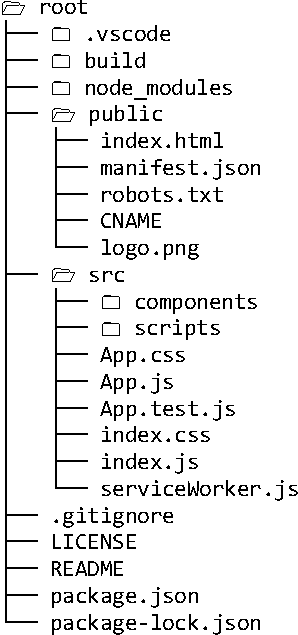
\includegraphics[width=0.25\textwidth]{obrazky-figures/adresarova_struktura.pdf}}
	    \caption{Adresářová struktura projektu.}
	    \label{obr:Adresářová struktura projektu}
    \end{figure}
        
    \item \textbf{src} -- V tomto adresáři je umístěna z~velké části samotná implementace aplikace jako jsou komponenty nebo skripty. Struktura není pevně daná, proto hierarchii podsložek lze libovolně upravovat pro lepší orientaci.
        \begin{itemize}
            \item \textbf{components} -- Zde jsou umístěny komponenty aplikace, které tvoří logický strom (více o~dekompozici komponent v~následující kapitole~\ref{sec:Dekompozice aplikace}).
            \item \textbf{scripts} -- Obsahuje skripty nutné pro běh aplikace, patří sem např. generátor shellu, logika transformace, web worker atd.
            \item \textbf{App.js} -- Komponenta na nejvyšší úrovní, ze které se větví další komponenty umístěné v~adresáři \texttt{components}.
            \item \textbf{index.js} -- Slouží jako \uv{brána} mezi stromem komponent vzniklý z~kořene \texttt{App.js} a \texttt{root} elementem v~souboru \texttt{index.html}.
            \item \textbf{serviceWorker.js} -- Je skript~\cite{website:ServiceWorkers} běžící na pozadí, oddělený od webové stránky a~otvírá dveře funkcím, které nevyžadují interakci s~webovou stránkou nebo uživatelem. Dnes obsahuje funkce jako jsou rozesílání push notifikací, chytrá práce s~mezipamětí prohlížeče, synchronizace na pozadí aj. V aplikaci je tento skript vygenerován, nezměněn a~nezaregistrován, jde spíše o~doplnění pro budoucí použití.
        \end{itemize}
    \item \textbf{package.json} -- Slouží nejen pro ukládání přímých závislostí na balíčcích, ale také usnadňuje jejich správu a~instalaci. Nachází se zde i~další metadata projektu jako je jméno aplikace, verze, licence apod. Zajímavou sekcí je sekce se skripty, která umožňuje definovat vlastní příkazy pro NPM, které byly využity například při nasazení aplikace (viz kapitola o~nasazení~\ref{sec:Nasazení aplikace}).
    \item \textbf{package-lock.json} -- Je automaticky generovaný soubor NPM při modifikaci \newline\texttt{node\_modules} nebo \texttt{package.json}, který obsahuje přesný strom závislostí verzí, to zaručuje shodné závislosti pro další programátory a~definuje chování programu. Ve výchozím nastavení \texttt{package.json} obsahuje pouze přímé závislosti, nikoliv závislosti závislostí, proto i~když zamkneme strom přímých závislostí není zaručeno, že plný strom bude identický. Vhodné je ponechat tento soubor ve správě NPM a~manuálně do něj nezasahovat.
\end{itemize}

\section{Dekompozice aplikace}
\label{sec:Dekompozice aplikace}
Dekompozice aplikace do funkcionálních komponent Reactu je znázorněna ve stromové struktuře na obrázku~\ref{obr:Soustava komponent aplikace ve stromové struktuře}, kde jména jsou odvozena od názvů souborů v~projektu. Každá komponenta je zodpovědná za určitou část aplikace a~případně drží potřebná data. V téhle situaci může být na místě otázka, zda nepoužít některou z knihoven pro řízení stavu, které jsou součásti ekosystému Reactu, jako je například knihovna Redux. Když se podíváme znovu na obrázek~\ref{obr:Soustava komponent aplikace ve stromové struktuře} vidíme, že výška stromu je pouze 4 a~zároveň data potřebná přenášet napříč celou aplikací je relativně málo, proto zavedení tohoto dodatečného frameworku mi přišlo poměrně těžkopádné. V případě budoucí větší expanze aplikace (z~pohledu dat nebo výšky stromu) je možné knihovnu pro řízení stavu snadno přidat a~přesunout do ní tato data. Stručný popis ke komponentám je potom v~následujícím textu.
\begin{figure}[hbt]
	\centering
	\setlength{\fboxsep}{0pt}
	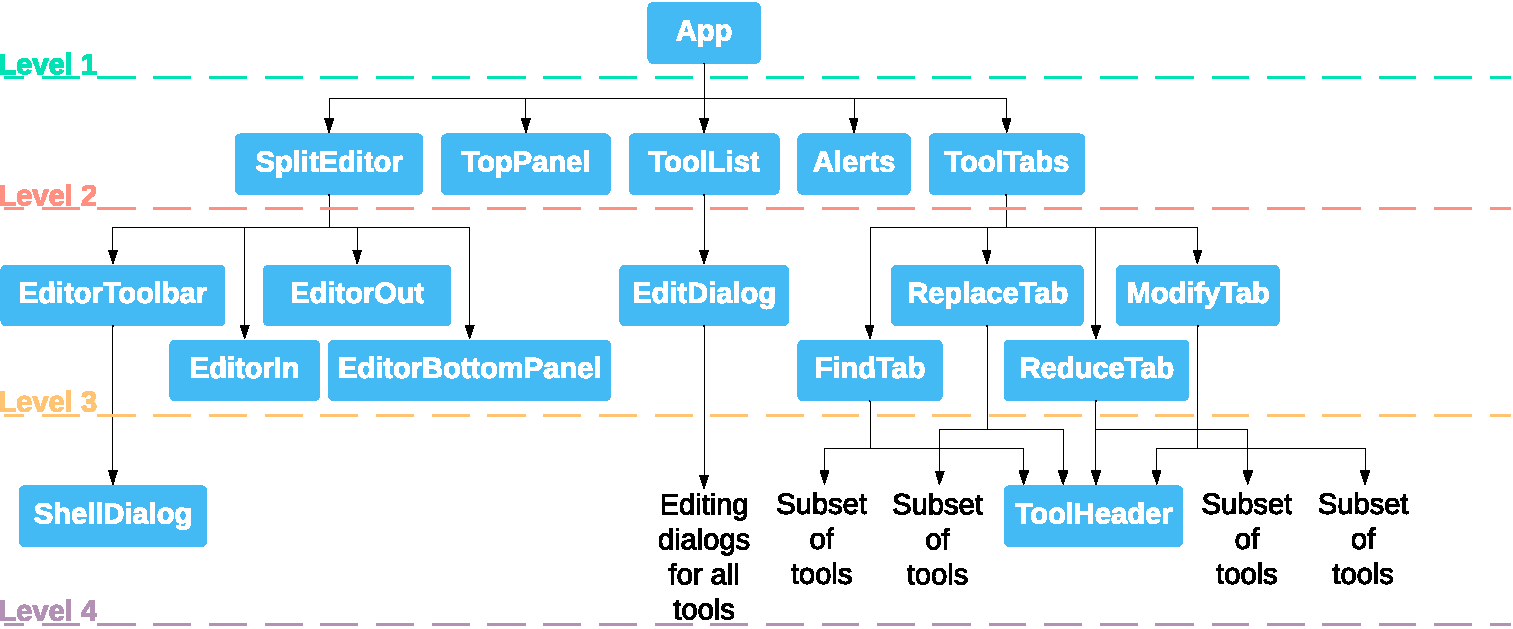
\includegraphics[width=1\textwidth]{obrazky-figures/dekompozice_komponent.pdf}
	\caption{Soustava komponent aplikace ve stromové struktuře. Každá komponenta obsahuje část rozhraní aplikace, případně drží potřebná data. Množina podobných komponent na listové úrovni je nahrazena textem kvůli jejich velkému počtu.}
	\label{obr:Soustava komponent aplikace ve stromové struktuře}
\end{figure}

\begin{itemize}
    \item \textbf{App} -- Jak již bylo zmíněno v~předchozí kapitole~\ref{sec:Struktura projektu} jedná se o~komponentu na nejvyšší úrovní a~jsou zde uložena zejména data potřebná napříč celou aplikací jako je např. seznam použitých nástrojů a~jejich konfigurace, protože pokud dvě a~více komponent potřebují určitá společná data, je potřeba tyto data definovat v~nejbližší, společné, nadřazené komponentě. Dále se zde nachází inicializace web workera a~správa potřebného kontextu pro provedení transformace (nastavení editoru, breakpointů aj.).
    \item \textbf{TopPanel} -- Obsahuje horní panel s~názvem aplikace a~menu.
    \item \textbf{SplitEditor} -- Slouží jako obálka pro editory. Nachází se zde nastavení zalamování řádků, přizpůsobení velikosti, ukazatel průběhu a~další.
    \item \textbf{EditorToolbar} -- Obsahuje panel nástrojů pro editor. Jsou zde stavy upřesňující nastavení hledaní pomocí regulárních výrazů nebo citlivost na velká písmena, jinak komponenta spíše využívá metody nadřazených komponent.
    \item \textbf{ShellDialog} -- Zde je definováno okno pro výpis shell skriptu pro provedení transformace na Linuxu. Samotné generování skriptu je pak provedeno v~souboru\newline \texttt{shellGenerator.js}, který je odtud zavolán.
    \item \textbf{EditorIn} -- Zahrnuje vstupní editor a~konfiguraci breakpointů.
    \item \textbf{EditorOut} -- Obsahuje výstupní editor. 
    \item \textbf{EditorBottomPanel} -- Komponenta pouze zobrazuje aktuální konfiguraci, která je ji předána a~neobsahuje žádný stav kromě aktuální pozice kurzoru v~editoru. Ačkoliv by bylo moudré, aby tento stav byl definován v~nadřazené komponentě a~následně byl pouze předán a~zobrazen. Místo toho je definován zde a~nastavení tohoto stavu je provedeno přes referenci z~nadřazené komponenty, což je proti dobrým zásadám programování tak, jak bylo zmíněno v~kapitole~\ref{sec:Komponenty}. V této situaci je problém, že pokud je vyvolána událost o~změně kurzoru z~komponenty editoru při editaci textu doprovázena událostí o~změně obsahu, vznikne požadavek na dvojí zpracování, provede se zápis pozice kurzoru, přepíše se komponenta a~obsah, který uživatel vložil bude ztracen. Proto, když je tento stav oddělen, může se pozice libovolně měnit bez ohledu na jiné události, protože stav je ovlivněn na jiných místech aplikace.
    \item \textbf{ToolList} -- V této části jsou použité nástroje namapovány do řaditelného seznamu, včetně popisu jejich konfigurace a~akcí, které s~nimi lze provádět. Zde je vhodné zmínit způsob generování položek, protože akce dostupné přes tlačítko vlastností (angl. \uv{properties}) potřebují vrchol, odkud se menu otevře. Zde však vzniká problém, protože list je generovaný během vykreslování a~vrchol je nutné znát ještě před jeho započetím. Důsledkem pak je situace, kdy se všechna menu vykreslují v~levém horním rohu monitoru (souřadnice \texttt{0,0}). Tento problém řeší externí knihovna \textbf{material-ui-popup-state\footnote{material-ui-popup-state: \url{https://github.com/jcoreio/material-ui-popup-state}}}, která nabízí vlastní hooky, které sledují stav těchto rolovacích elementů a~připojují k~nim spouštěcí funkce, které pak nasměrují vykreslené položky menu na správné místo.
    \item \textbf{EditDialog} -- Je dialogové okno dostupné přes seznam použitých nástrojů, které umožňuje zpětně editovat konfiguraci nástroje. V tomhle souboru je definován pouze abstrakt tohoto okna, který je společný pro všechny nástroje (popis, dialogové akce aj.). Samotný obsah je pak definován odpovídajícím nástrojem, který musí implementovat metodu \texttt{handleUpdate()}, která validuje platnost vstupů před potvrzením změn a~následně uzavře okno. Obsah je pro každý nástroj individuální a~tyto soubory jsou umístěny v~adresáři \texttt{/src/components/edits/tools}. Kvůli většímu počtu těchto souborů jsou na obrázku~\ref{obr:Soustava komponent aplikace ve stromové struktuře} tyto komponenty nahrazeny textem.
    \item \textbf{ToolTabs} -- Zde jsou definovány kategorie a~k~nim připojeny příslušné karty s~nástroji. Jde spíše o~abstrakt zajišťující navigaci a~přizpůsobení šířce monitoru pomocí \texttt{MeadiaQuery} stejně jako v~seznamu použitých nástrojů. Samotné karty s~kategoriemi potom importují nástroje z~adresáře \texttt{/src/components/tabs/tools}, kde opět na obrázku~\ref{obr:Soustava komponent aplikace ve stromové struktuře} jsou podmnožiny těchto nástrojů nahrazeny textem kvůli jejich počtu. Tato skutečnost umožňuje v~budoucnu pak snadno zaměňovat obsah jednotlivých kategorií editací jednoho řádku.
    \item \textbf{FindTab} -- Obsahuje nástroje, jejichž primárním účelem je hledání nebo porovnávání.
    \item \textbf{ReplaceTab} -- Poskytuje nástroje pro náhradu textu.
    \item \textbf{ReduceTab} -- Zde jsou nástroje, jejichž účelem je redukce textu.
    \item \textbf{ModifyTab} -- Obsahuje nástroje, které nějakým způsobem zaměňují nebo obohacují text.
    \item \textbf{ToolHeader} -- Je komponenta použita při definici každého nástroje a~poskytuje její název a~funkční popis. Výsledkem je pak jednotný styl pro všechny nástroje a~snížena redundance kódu.
    \item \textbf{Alerts} -- Zde jsou implementovány informační vyskakovací okna, která se zobrazují vlevo dole na monitoru po dobu 2 sekund. Jde primárně o~sdělující animaci, takže spouštěcí akce je provedena přes referenci. Zpracování požadavku na zobrazení sdělení je zařazeno na konec fronty a~obsluha je pak provedena následovně:
    \begin{itemize}
        \item Je-li fronta prázdná zobrazí se sdělení ihned.
        \item Pokud je sdělení aktuálně zobrazeno, zavře se a~zobrazí se následující.
        \item Není-li zobrazeno žádné sdělení a~fronta je neprázdná, zařadí se požadavek na její konec.
    \end{itemize}
\end{itemize}

\section{Proces zpracování textu}
Data potřebná ke zpracování včetně samotného procesu se nachází v~komponentě na nejvyšší úrovni a~transformaci je potřeba provést automaticky vždy, když uživatel provede akci, která ovlivňuje výsledek. Jedná se tedy o~následující události:
\begin{itemize}
    \item Změní se obsah editoru (se zpožděním 1,5 sekundy kvůli optimalizaci výkonu)
    \item Přepnutí režimu editoru
    \item Manipulace s~breakpointy
    \item Přidání nástroje
    \item Editace nástroje
    \item Smazání nástroje
    \item Aktivace nebo deaktivace nástroje
    \item Změna pořadí nástrojů
\end{itemize}
\definecolor{ao}{rgb}{0.0, 0.5, 0.0}
\definecolor{amber}{rgb}{1.0, 0.49, 0.0}
\lstdefinelanguage{JavaScript}{
  keywords={const, typeof, new, true, false, catch, function, return, null, catch, switch, var, if, in, while, do, else, case, break},
  keywordstyle=\color{blue}\bfseries,
  ndkeywords={class, export, boolean, throw, implements, import, this, worker, useEffect},
  ndkeywordstyle=\color{amber}\bfseries,
  identifierstyle=\color{black},
  sensitive=false,
  comment=[l]{//},
  morecomment=[s]{/*}{*/},
  commentstyle=\color{ao}\ttfamily,
  stringstyle=\color{red}\ttfamily,
  morestring=[b]',
  morestring=[b]"
}
\lstset{
    language=JavaScript,
    basicstyle=\ttfamily\small,
    numberstyle=\footnotesize,
    numbers=left,
    frame=single,
    tabsize=2,
    rulecolor=\color{black!30},
    title=\lstname,
    escapeinside={\%*}{*)},
    escapechar={|},
    breaklines=true,
    breakatwhitespace=true,
    framextopmargin=2pt,
    framexbottommargin=2pt,
    extendedchars=false,
    inputencoding=utf8,
}
\begin{lstlisting}[caption={Komunikační cyklus zpracování textu. Na začátku je vytvořena instance web workera, kterému je zaslána zpráva s~potřebnými daty ke zpracování. Následně je definované chování na příchozí odpovědi. V poslední fázi je provedeno jeho ukončení.}, label={vyp:Komunikační cyklus ke zpracování textu}]
useEffect(() => {
    const worker = new WebWorker(pipeWorker);   // Vytvoreni web workera

    worker.postMessage({                        // Odeslani zpravy s daty ke zpracovani
        text: editorContent, 
        pipeline: pipeline, 
        breakpoints: inspectMode.breakpoints, 
        inspectMode: inspectMode.enabled
    });

    worker.onmessage = (event) => {             // Definice reakci na odpovedi
        if (event.data.type === "progress") {
            setPipeProgress(event.data.data);       // Zobrazeni postupu zpracovani
        }
        else {
            setEditorResult(event.data.data);       // Vypis vysledku
        }
    };

    return () => {                              // Uklid
        worker.terminate();                     // Ukonceni workera
    };
}, [editorContent, pipeline, inspectMode]);
\end{lstlisting}
Klíčová část kódu pro zpracování textu, která pracuje s~web workerem je zobrazena na výpisu~\ref{vyp:Komunikační cyklus ke zpracování textu}. Zpracování se provádí v~metodě \texttt{useEffect()}, která je podrobněji popsána v~kapitole~\ref{sec:Životní cyklus komponent a React hooks}. Dojde-li ke změně stavu, není změna hned dostupná, ale stav se změní asynchronně později, protože React v~daný moment ještě chvíli vyčkává na další případné změny stavů a~poté všechny tyto změny provede naráz. Tato metoda je tedy zavolána potom, co už jsou tyto změny provedeny a~platné.

Přesněji stavy, které jsou sledovány touto metodou jsou definovány na řádku~23 a~jedná se o~vstup editoru, použité nástroje a~strukturu s~ladícími daty. Jako první se inicializuje web worker a~je mu zaslána zpráva s~potřebnými daty ke zpracování textu. Tedy jedná se o~řetězec vstupního textu, list s~konfigurací použitých nástrojů, list breakpointů a~boolovská hodnota stavu ladícího režimu. Následně na řádku~11 je definovaná reakce na odpovědi, kde se buď zobrazuje postup během procesu zpracování nebo se vypíše výsledek. Na závěr na řádku~20 je provedeno uvolnění alokovaných zdrojů, které se provede při odpojení (poslední fázi), aby na pozadí neběžely předešlé skripty workerů. Celý proces se pak při novém požadavku na zpracování opakuje.

Logika zpracování textu ze strany workera po přijetí požadavku s~potřebnými parametry je znázorněna v~algoritmu~\ref{alg:Proces zpracování textu}. V případě ladícího režimu, kde je požadována transformace typicky nad malém množství záznamů, je transformace provedena také nad celými daty a~poté jsou tyto požadované části vyselektovány, jelikož některé nástroje vyžadují znalost okolních záznamů (kontext) a~jen aktuální záznam nestačí. Zároveň některé nástroje zaměňují jejich pořadí či je jinak modifikují, proto je nutné každý záznam očíslovat, aby byl nakonec dohledatelný. Na začátku algoritmu je provedeno zpracování vstupního textu do vhodné podoby. V případě ladícího režimu je text uložen do struktury, kde každý záznam obsahuje data a~právě dané číslo. V běžném režimu postačí text jako klasický řetězec. Dále je definován přírůstek na ukazateli průběhu, který bude odeslán po zpracování každého použitého nástroje. Následuje zpracování všech aktivních nástrojů postupně za sebou nad celým textem. Výsledek z~každého nástroje je pak předán následujícímu. Zde je opět nutné rozlišit způsob zpracování, které se buď provádí nad řetězcem nebo nad strukturou. V případě dat uložených ve struktuře je záznam, který není obsažen ve výsledku označen klíčovým slovem \texttt{null}. Po zpracování celého textu je výsledek odeslán zpět do aplikace. V případě ladícího režimu je nutné ještě předem výsledná data ze struktury extrahovat pomocí čísel řádků, nad kterými jsou nastavené breakpointy a~vytvořit z~nich řetězec.

\begin{algorithm}
\caption{Proces zpracování textu}
\label{alg:Proces zpracování textu}
\begin{algorithmic}[1]
\Procedure{ProcessPipeline}{$text,pipeline, breakpoints, inspectMode$}
    \If{$inspectMode$ == \texttt{false}} \Comment{Načtení textu}
        \State $data \gets text$
    \Else \Comment{Označení řádků pomocí struktury}
        \State $i \gets 0$
        \ForEach {$line \in text$}
            \State $data[i] \gets$ \{number: $i + 1$, data: $line$\}
            \State $i \gets i + 1$
        \EndFor
    \EndIf
    \State $unit \gets$ 100 / len($pipeline$)
    \If{len($pipeline$) $> 0$}
        \State postMessage(\{type: $"progress"$, data: $0$\}) \Comment{Informace o procesu zpracování}
    \EndIf
    \State $i \gets 0$
    \ForEach {$tool \in pipeline$} \Comment{Zpracování nástrojů}
        \If{$tool$.active() == \texttt{true}}
            \If{$inspectMode$ == \texttt{false}}
                \State $data \gets$ processTool($data, tool$)
            \Else
                \State $data \gets$ processInspectTool($data, tool$)
            \EndIf
        \EndIf
        \State postMessage(\{type: $"progress"$, data: $(i + 1) * unit$\})
        \State $i \gets i + 1$
    \EndFor
    \If{$inspectMode$ == \texttt{true}} \Comment{Extrakce dat ze struktury}
        \State $temp \gets$ empty list
        \ForEach{$line \in data$}
            \If{$breakpoints$.includes($line$.number) \texttt{\&\&} $line$.data != \texttt{null}}
                \State $temp$.append($line$.data)
            \EndIf
        \EndFor
        \State $data \gets temp$.join('\textbackslash{}n')
    \EndIf
    \State postMessage(\{type: $"result"$, data: $data$\}) \Comment{Odeslání výsledku}
\EndProcedure
\end{algorithmic}
\end{algorithm}

\section{Tvorba automatizovaných testů}
Testy byly vytvořeny samostatně od hlavního projektu a~byly implementovány v~Pythonu~3.6 na frameworku Selenium (viz kapitola~\ref{sec:Selenium}) s~BDD scénáři (viz kapitola~\ref{sec:Automatické testování}). Struktura adresáře testů je znázorněna na obrázku~\ref{obr:Adresářová struktura testů}, kde v~adresáři \texttt{drivers} jsou umístěny potřebné ovladače k~ovládání prohlížeče. Při testování byl použit ovladač pro Firefox GeckoDriver\footnote{GeckoDriver: \url{https://github.com/mozilla/geckodriver/releases}}. V adresáři \texttt{features} jsou napsány všechny testovací scénáře, jejichž kroky jsou pak implementovány v~adresáři \texttt{features/steps}. Důležitým souborem je soubor \texttt{environment.py}, ve kterém je provedeno nastavení prostředí před spuštěním testů (volba prohlížeče, ovladače, doba čekání atd.) a~úklid po jejich provedení.
\begin{figure}[hb]
	\centering
	\setlength{\fboxsep}{4pt}
	\fbox{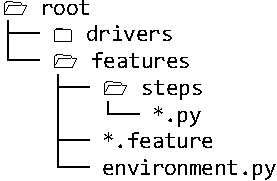
\includegraphics[width=0.35\textwidth]{obrazky-figures/selenium_struktura.pdf}}
	\caption{Adresářová struktura testů.}
	\label{obr:Adresářová struktura testů}
\end{figure}
\lstdefinelanguage{gherkin}
{
  morekeywords={
    Feature,
    Scenario,
    Given,
    When,
    Then,
    And
  },
  sensitive=false,
  morestring=[b]"
}
\definecolor{eclipsePurple}{RGB}{127,0,85}
\lstset{
    language={gherkin},
    basicstyle=\ttfamily\small,
    numberstyle=\footnotesize,
    numbers=left,
    frame=single,
    tabsize=2,
    rulecolor=\color{black!30},
    title=\lstname,
    escapeinside={\%*}{*)},
    escapechar={|},
    breaklines=true,
    breakatwhitespace=true,
    framextopmargin=2pt,
    framexbottommargin=2pt,
    extendedchars=false,
    keywordstyle=\color{eclipsePurple},
    inputencoding=utf8,
}
\begin{lstlisting}[caption={Testovací scénáře v~jazyce Gherkin.}, label={vyp:Testovací scénáře}]
Feature: Editor
    
    Scenario: Krok zpet
        Given Uzivatel se nachazi na strance weboveho nastroje
        And Do vstupniho editoru je vlozeno "text"
        When Uzivatel vrati krok zpet
        Then Vstupni editor obsahuje ""
        
    Scenario: Krok dopredu
        Given Uzivatel se nachazi na strance weboveho nastroje
        And Do vstupniho editoru je vlozeno "text"
        When Uzivatel vrati krok zpet
        And Uzivatel se vrati krokem dopredu
        Then Vstupni editor obsahuje "text"
\end{lstlisting}
Příklad testovacího scénáře je zobrazen na výpisu~\ref{vyp:Testovací scénáře}, kde:
\begin{itemize}
    \item \texttt{Feature} -- Je abstraktní popis následující skupiny scénářů.
    \item \texttt{Scenario} -- Obsahuje název testovacího případu.
    \item \texttt{Given} -- Definuje počáteční kontext před provedením testu, tedy to, co musí být nastaveno před zahájením.
    \item \texttt{When} -- Jsou kroky popisující události provedeny interakcí uživatele s~aplikací.
    \item \texttt{Then} -- Popisuje očekávaný výsledek.
    \item \texttt{And} -- Je klíčové slovo, které dědí funkcionalitu předešlého pro plynulé strukturovaní. Např. při použití více akcí \texttt{Then} jej definujeme pouze jednou a~následně používáme slovo \texttt{And}.
\end{itemize}
Pro automatizaci běhů testů je použit program Behave\footnote{Behave: \url{https://behave.readthedocs.io/en/latest}}, který lze spustit příkazem \texttt{behave} v~kořenovém adresáři projektu po správné konfiguraci potřebných závislostí. Program poté začne vyhledávat \texttt{.feature} soubory s~testovacími scénáři v~adresáři \texttt{features} a~jejich implementované kroky v~adresáři \texttt{features/steps}, proto je nutné zachovat tuto adresářovou strukturu. Výpis výsledků je pak zobrazen na obrázku~\ref{obr:Výsledky testů}.
\begin{figure}[hbt]
	\centering
	\setlength{\fboxsep}{0pt}
	\fbox{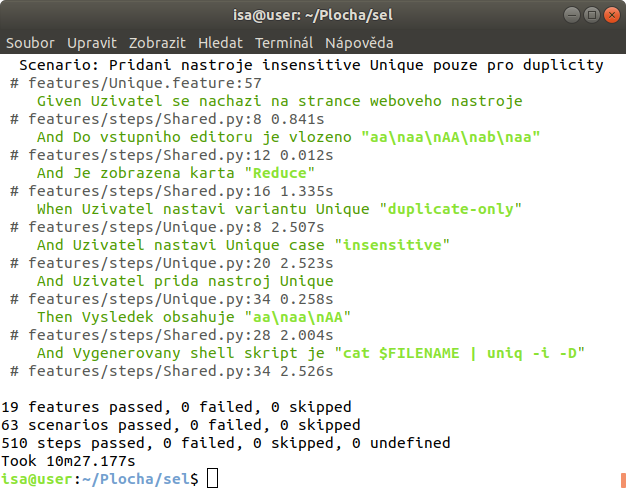
\includegraphics[width=0.8\textwidth]{obrazky-figures/vypis_testu.png}}
	\caption{Výsledky implementovaných testů.}
	\label{obr:Výsledky testů}
\end{figure}

\section{Nasazení aplikace}
\label{sec:Nasazení aplikace}
Aplikace\footnote{Craftex: \url{https://craftex.app}} byla zveřejněna pomocí služby GitHub Pages (viz kapitola~\ref{sec:GitHub Pages}), kvůli které byla přidána další knihovna \texttt{gh-pages}\footnote{gh-pages: \url{https://www.npmjs.com/package/gh-pages}}, která usnadňuje a~automatizuje proces nasazení. Nasazení sestavené aplikace je provedeno ve zvláštní větvi GitHub repozitáře projektu pro gh-pages, odkud bude aplikace dostupná. Samotná konfigurace skriptů pro nasazení je znázorněna na výpisu~\ref{vyp:Konfigurace skriptů} a~nachází se v~souboru \texttt{package.json}. Nasazení lze pak provést přes terminál v~kořenovém adresáři projektu příkazem \texttt{npm run deploy}, který vloží sestavenou aplikaci na web z~adresáře \texttt{build}. Ovšem před provedením této operace je automaticky spuštěn příkaz \texttt{predeploy}, který obsahuje skript \texttt{npm run build} pro sestavení aplikace. Odkaz, přes který bude aplikace dostupná je definován na řádku 1 (viz výpis~\ref{vyp:Konfigurace skriptů}), jinak by se aplikace nezobrazovala korektně, přesněji by se zobrazilo pouze bíle okno.

% Inspirováno: https://tex.stackexchange.com/questions/83085/how-to-improve-listings-display-of-json-files
\colorlet{punct}{red!60!black}
\definecolor{background}{HTML}{EEEEEE}
\definecolor{delim}{RGB}{20,105,176}
\colorlet{numb}{magenta!60!black}
\lstdefinelanguage{json}{
    basicstyle=\normalfont\ttfamily,
    numbers=left,
    numberstyle=\scriptsize,
    stepnumber=1,
    numbersep=8pt,
    showstringspaces=false,
    breaklines=true,
    frame=single,
    literate=
     *{0}{{{\color{numb}0}}}{1}
      {1}{{{\color{numb}1}}}{1}
      {2}{{{\color{numb}2}}}{1}
      {3}{{{\color{numb}3}}}{1}
      {4}{{{\color{numb}4}}}{1}
      {5}{{{\color{numb}5}}}{1}
      {6}{{{\color{numb}6}}}{1}
      {7}{{{\color{numb}7}}}{1}
      {8}{{{\color{numb}8}}}{1}
      {9}{{{\color{numb}9}}}{1}
      {:}{{{\color{punct}{:}}}}{1}
      {,}{{{\color{punct}{,}}}}{1}
      {\{}{{{\color{delim}{\{}}}}{1}
      {\}}{{{\color{delim}{\}}}}}{1}
      {[}{{{\color{delim}{[}}}}{1}
      {]}{{{\color{delim}{]}}}}{1},
}

\begin{lstlisting}[language=json, caption={Konfigurace skriptů}, label={vyp:Konfigurace skriptů}]
"homepage": "https://craftex.app",
"scripts": {
    "predeploy": "npm run build",
    "deploy": "gh-pages -d build",
    "start": "react-scripts start",
    "build": "react-scripts build",
    "test": "react-scripts test",
    "eject": "react-scripts eject"
},
\end{lstlisting}

Vždy před nasazením aplikace byla provedena bezpečnostní revize příkazem \texttt{npm audit}, který hledá zranitelnosti projektu ve stromu závislostí. Pokud jsou detekovány nějaké chyby, lze je někdy opravit automaticky příkazem \texttt{npm audit fix} (případně opakovaně, protože opravení některých chyb může napomoci opravení jiných, dříve automaticky neopravitelných), v~opačném případě je nutné provést opravu ručně.

Doména aplikace byla zvolena s~příponou \texttt{.app} za cenu $435$~Kč/rok, která je určena především pro aplikace a~vyžaduje aplikační protokol HTTPS, který zároveň služba GitHub Pages podporuje. Kromě nastavení DNS záznamů je nutné do kořenového adresáře sestavené aplikace umístit soubor s~názvem \texttt{CNAME} obsahující doménu aplikace, aby se GitHub mohl na aplikaci  pomocí této domény odkázat.

\section{Výsledná podoba aplikace}
\label{sec:Výsledná podoba aplikace}
Na obrázku~\ref{obr:Výsledná podoba aplikace} je zobrazena výsledná podoba aplikace. V horní liště se nachází záložky s~funkcemi rozdělené do kategorií pro soubory, editor, použité nástroje a~vyhledávač, který je společný pro vstupní i~výstupní editor. Taktéž je možno použít klávesovou zkratku  \uv{ctrl + F} v~každém editoru separátně. Velikost editorů lze měnit do výšky i~do šířky a~ladění je realizováno pomocí breakpointů (například řádek~$111\,241$ na obrázku~\ref{obr:Výsledná podoba aplikace}). Těsně pod editory se nachází modrá lišta zobrazující stav při převodu. Dále se pod ní nachází lišta s~informacemi o~aktuálním nastavení editoru. Zhruba uprostřed aplikace se nachází sekce pojmenovaná anglicky \uv{pipeline}, která zobrazuje aktuálně použité nástroje. Každý nástroj je možné dodatečně editovat (viz dialogové okno na obrázku~\ref{obr:Editace použitého nástroje}), deaktivovat nebo odstranit. Zpracování je prováděno shora dolů a~pořadí je možné libovolně zaměňovat prostým přetažením. Velikost této sekce je taktéž možné měnit do výšky. Pomocí dialogového okna je také zobrazován shell skript, který je možné vidět na obrázku~\ref{obr:Zobrazení shell skriptu}. V poslední části se nachází galerie nástrojů rozdělena do kategorií podle primárního účelu pro usnadnění orientace. V případě chybně zadaných parametrů je uživatel upozorněn hláškou a~zvýrazněním příslušného vstupu. Každý nástroj obsahuje funkční popis, který slouží jako manuálová stránka. Celý návrh je responzivní a~použitelný i~na mobilních zařízeních (viz obrázek~\ref{obr:Mobilní zobrazení}). Hlavní změnou na mobilním zařízení je eliminace odsazení od krajů prohlížeče a~poskytnutí tak více prostoru pro vstupy, zároveň dialogová okna jsou zobrazována přes celé okno zařízení. Ostatní funkcionalita zůstává zachována a~při použití zařízení na šířku je pak práce s~aplikací z~mého pohledu ještě jednodušší. Výslednou podobu lze také vidět na vytvořeném demonstračním videu\footnote{Demo: \url{https://youtu.be/KA4wxr-8vKk}} dostupném na internetovém portálu YouTube.
\begin{figure}[hbt]
	\centering
	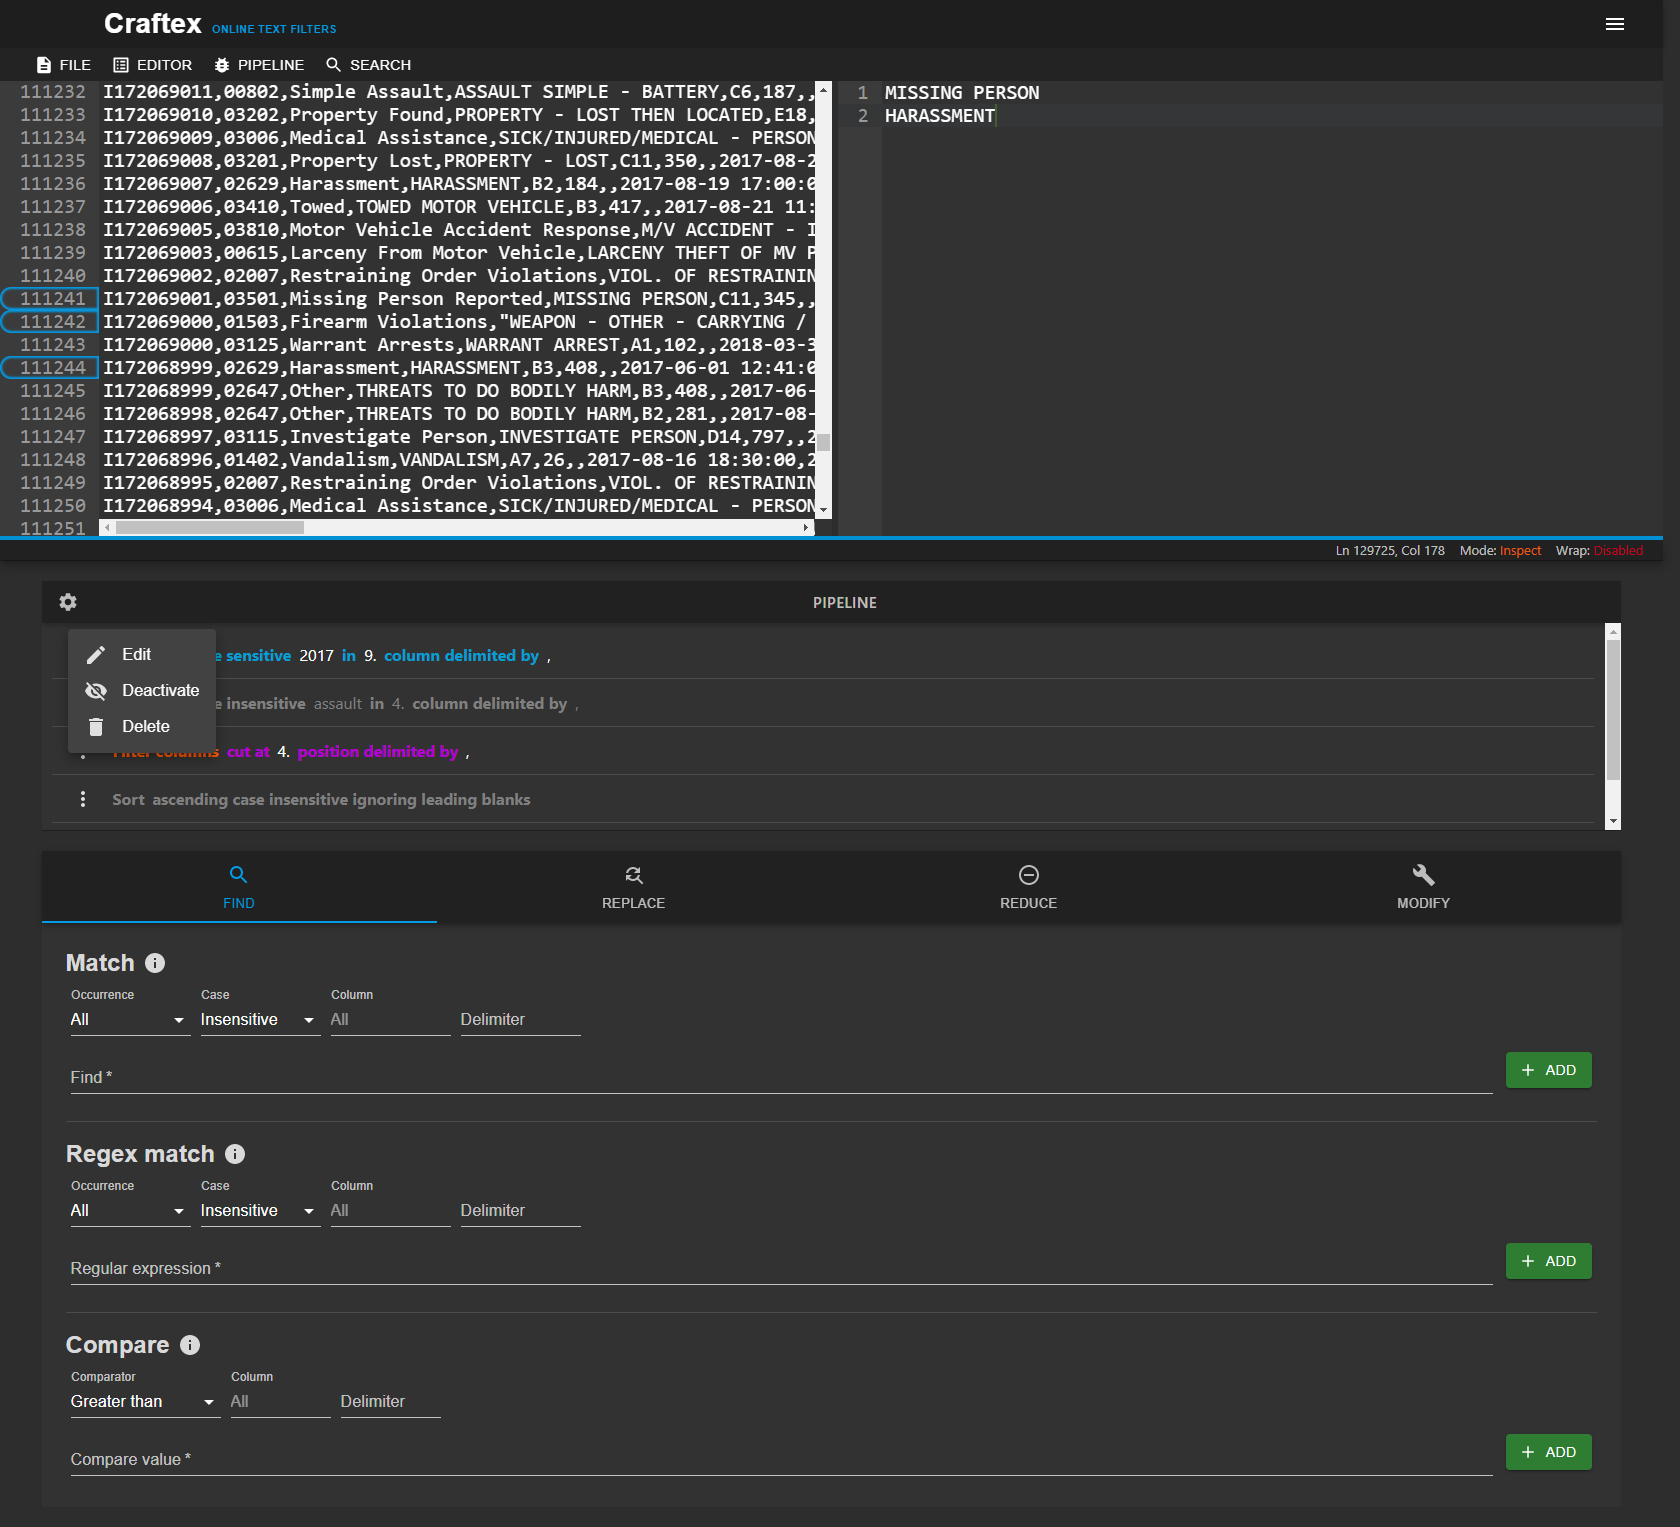
\includegraphics[width=0.98\textwidth]{obrazky-figures/vysledna_podoba.png}
	\caption{Výsledná podoba aplikace.}
	\label{obr:Výsledná podoba aplikace}
\end{figure}
\begin{figure}[hbt]
	\centering
	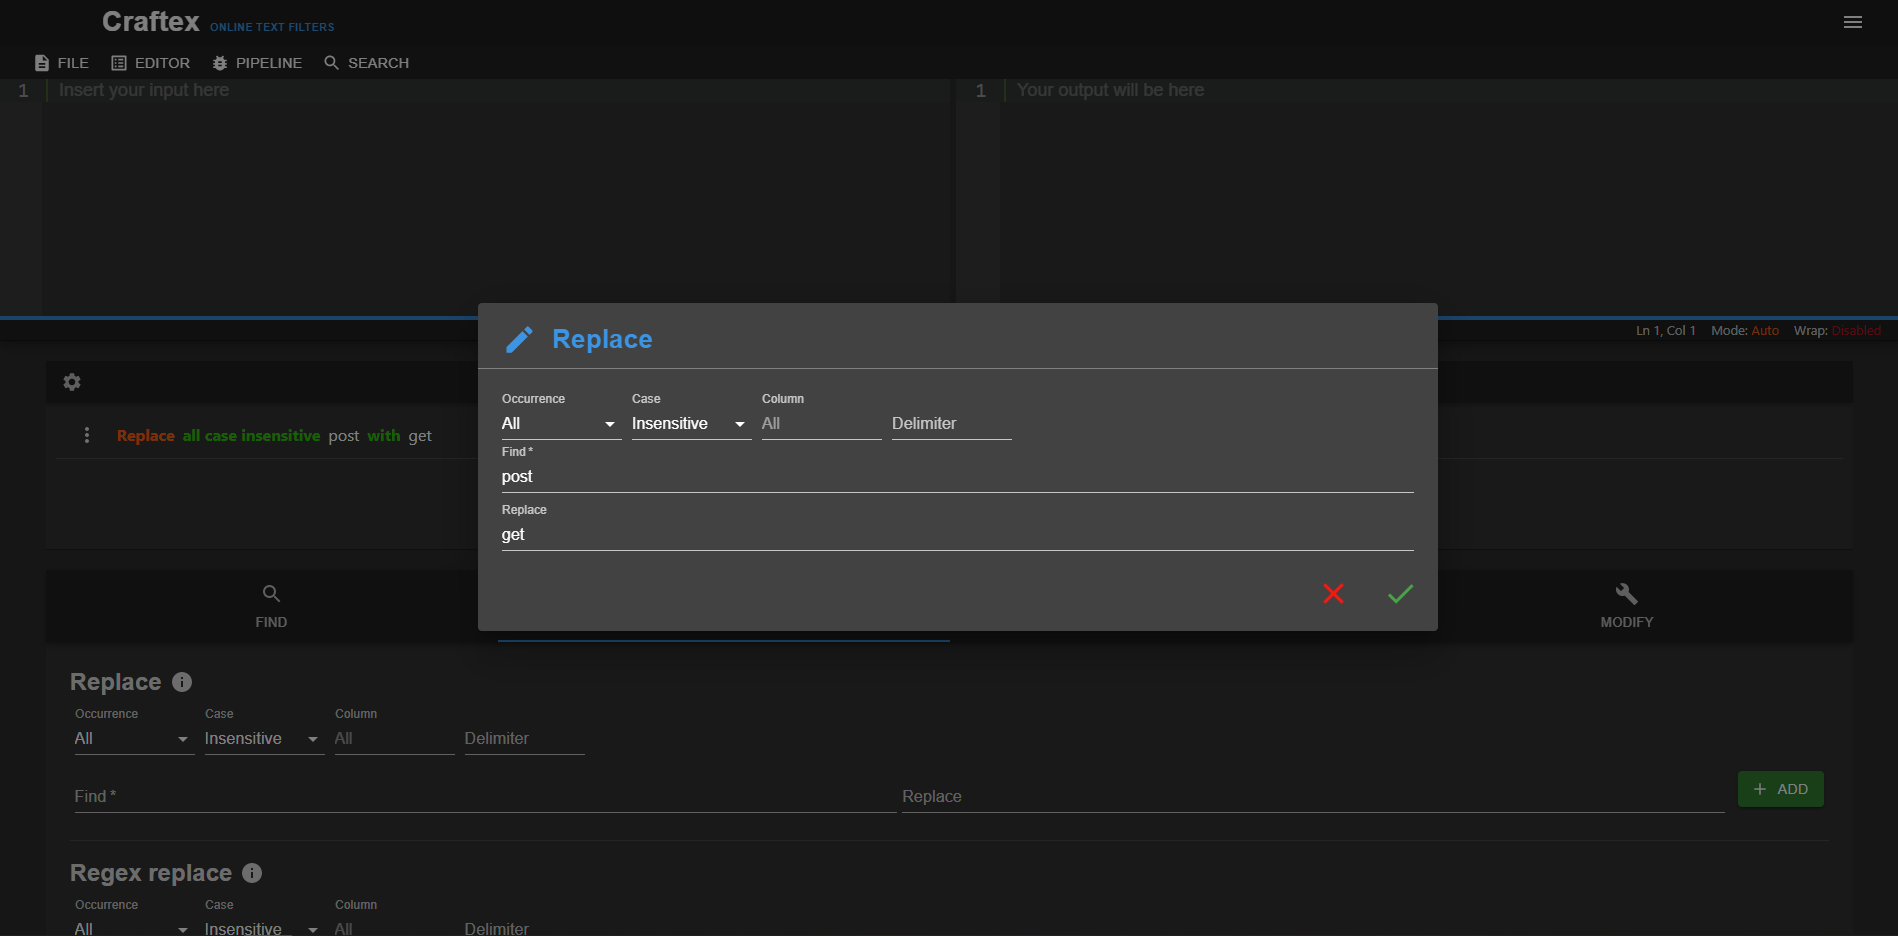
\includegraphics[width=0.98\textwidth]{obrazky-figures/editace_nastroje.PNG}
	\caption{Editace použitého nástroje.}
	\label{obr:Editace použitého nástroje}
\end{figure}
\begin{figure}[hbt]
	\centering
	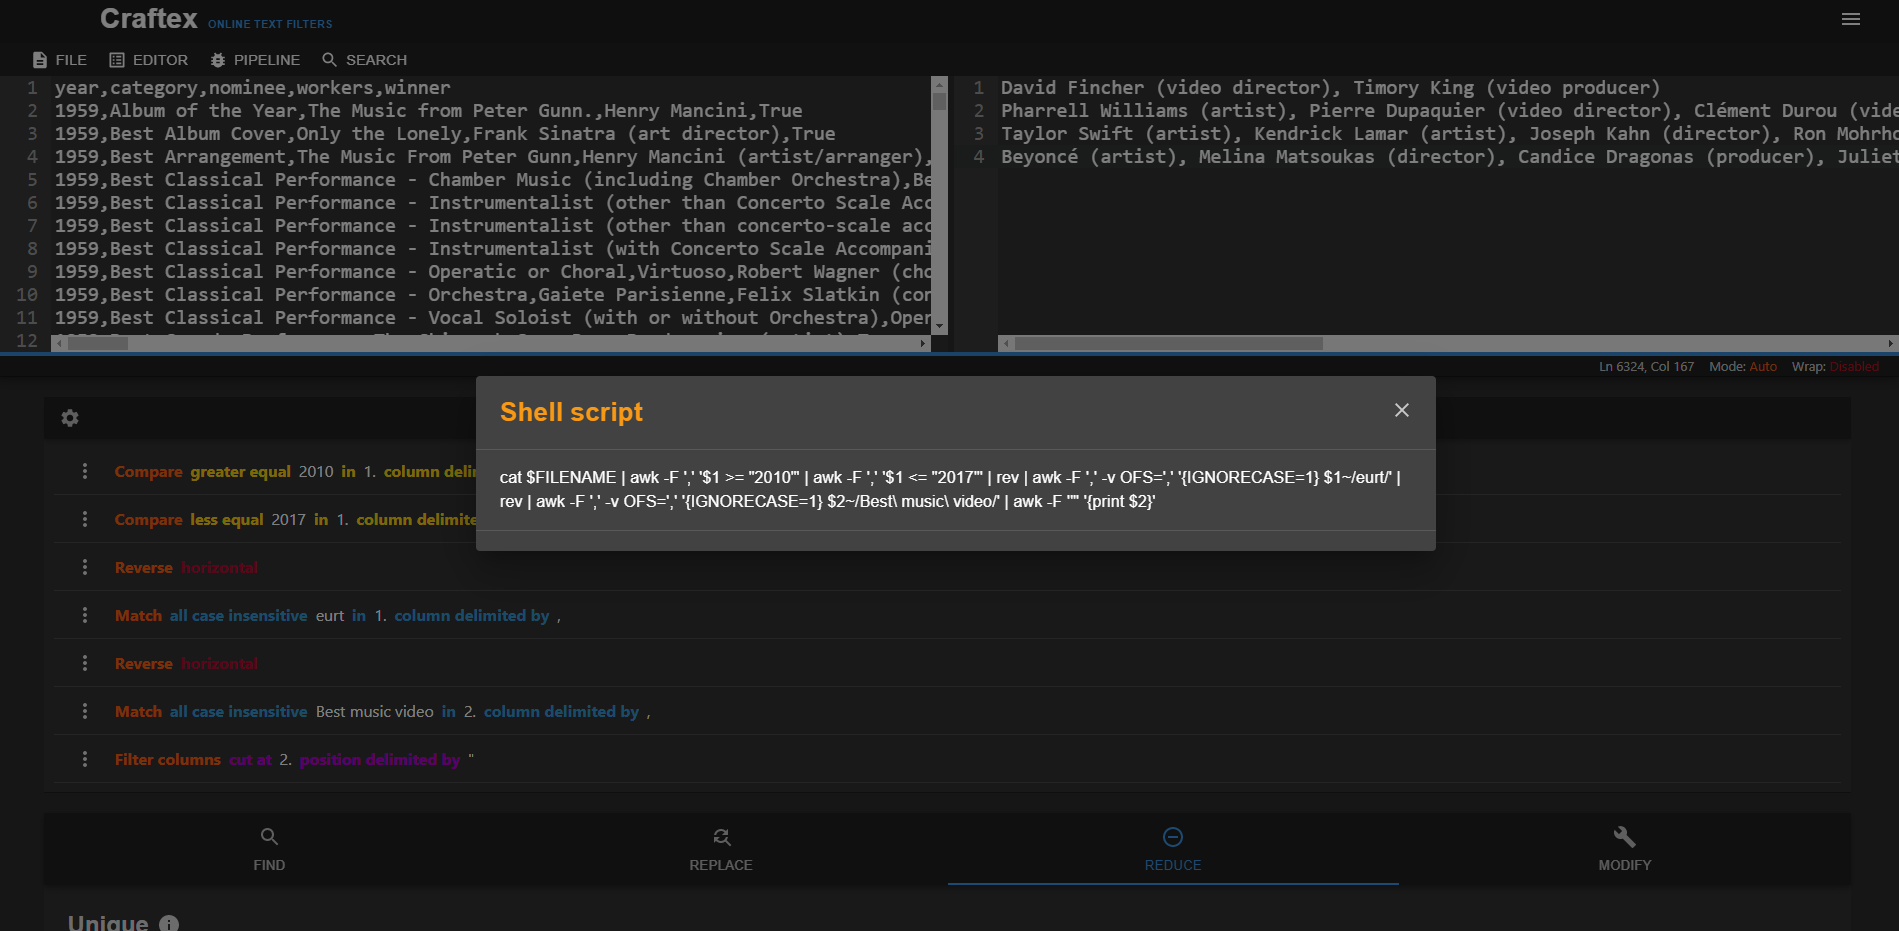
\includegraphics[width=1\textwidth]{obrazky-figures/shell_dialog.PNG}
	\caption{Zobrazení vygenerovaného shell skriptu.}
	\label{obr:Zobrazení shell skriptu}
\end{figure}
\begin{figure}[hbt]
	\centering
	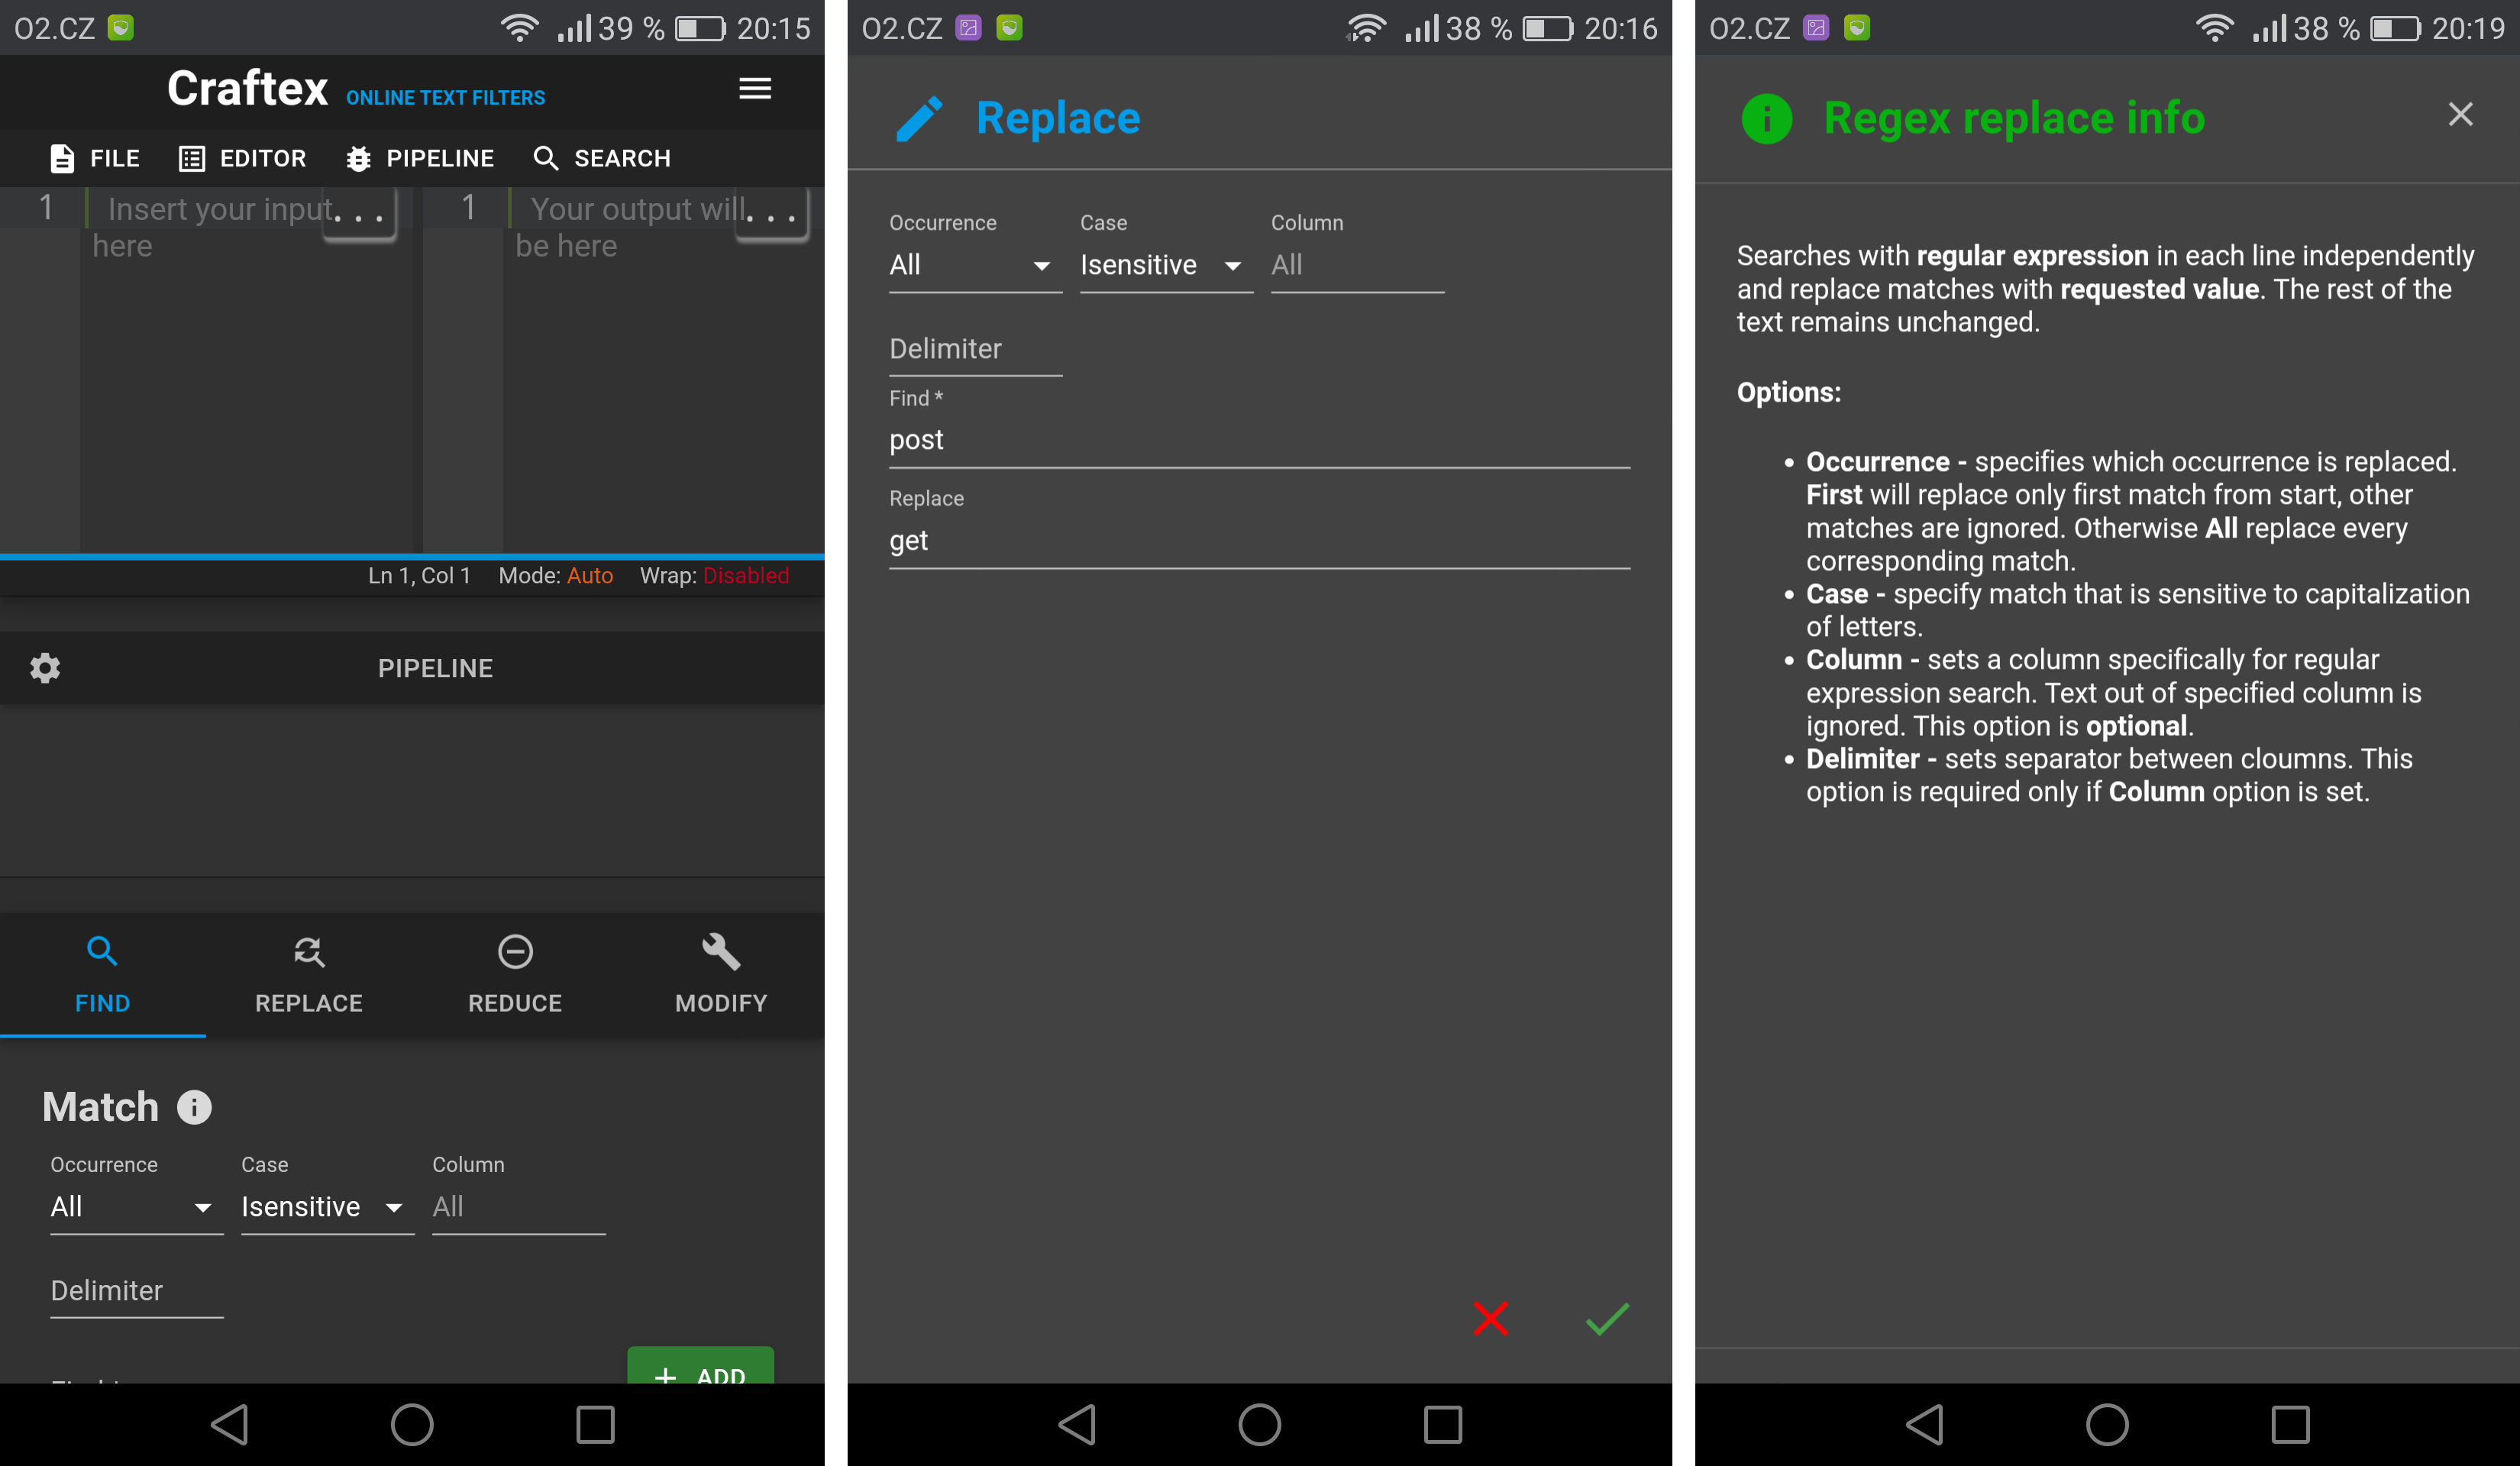
\includegraphics[width=1\textwidth]{obrazky-figures/mobilni_verze.png}
	\caption{Aplikace na mobilním zařízení. V levé části je zobrazena hlavní stránka aplikace, uprostřed se nachází editace nástroje a~vpravo je zobrazen funkční popis nástroje.}
	\label{obr:Mobilní zobrazení}
\end{figure}

%=========================================================================
\chapter{Sběr dat a testování}
\label{chap:Sběr dat a testování}
V této kapitole je zmíněna testovací datová sada a~hlavní zdroje, ze kterých byla pořízena, včetně ukázek její filtrace. Další část je věnována metodice provedeného automatizovaného testování. Poslední část obsahuje uživatelské testování, kde se uživatelé podíleli svoji zpětnou vazbou na doladění aplikace a~je také zmíněn výsledek provedeného časového testu, jehož cílem bylo zhodnotit efektivitu výsledného řešení.

\section{Testovací datová sada}
Během procesu implementace byla shromažďována reálná vstupní data vhodná k~filtraci, která byla použita zejména při uživatelském testování a~prezentaci aplikace. Nejčastěji byla data získávaná od ostatních uživatelů, z~různých míst operačního systému nebo z~následujících portálů:
\begin{itemize}
    \item \textbf{Kaggle\footnote{Kaggle: \url{https://www.kaggle.com}}} -- Dceřiná společnost společnosti Google, která poskytuje datové sady z~různých oborů vědy a~od odborníků na strojové učení.
    \item \textbf{DataHub\footnote{DataHub: \url{https://datahub.io}}} -- Je portál poskytující kolekce dat z~různých zdrojů ve formě architektury hub.
    \item \textbf{Data.gov\footnote{Data.gov: \url{https://www.data.gov}}} -- Je americká vládní stránka poskytující hodnotné informace z~federální, vládní a~státní oblasti pro širokou veřejnost.
\end{itemize}
Celkem bylo nasbíráno přes $60$~různých exemplářů s~celkovou velikostí přes $200$~MB. Možné případy takto vyfiltrovaných dat jsou znázorněny níže.

\subsection*{1. ukázka}
Data byla pořízena ze školního serveru Merlin, ze kterých jsou vyfiltrováni uživatelé, kteří mají spuštěnou instanci textového editoru \texttt{vim}, včetně časového údaje, kdy byl proces spuštěn. Filtrace je znázorněna na obrázku~\ref{obr:Filtrace1}, fragment vstupních dat na výpisu~\ref{vyp:vstup1} a~fragment výstupních dat na výpisu~\ref{vyp:vystup1}.

\clearpage
\begin{lstlisting}[caption={Fragment vstupních dat.}, label={vyp:vstup1}]
USER       PID %CPU %MEM    VSZ   RSS TTY      STAT START   TIME COMMAND
root         1  0.0  0.0 192848  6692 ?        Ss   led22  82:50 /usr/lib/systemd/systemd --system --deserialize 22
root         2  0.0  0.0      0     0 ?        S    led22   0:28 [kthreadd]
\end{lstlisting}

\begin{lstlisting}[language=TeX, caption={Fragment výstupních dat.}, label={vyp:vystup1}]
xkubov06 úno18 
xbegan01 12:34 
xmjach00 12:35 
\end{lstlisting}

\begin{figure}[hbt]
	\centering
	\setlength{\fboxsep}{0pt}
	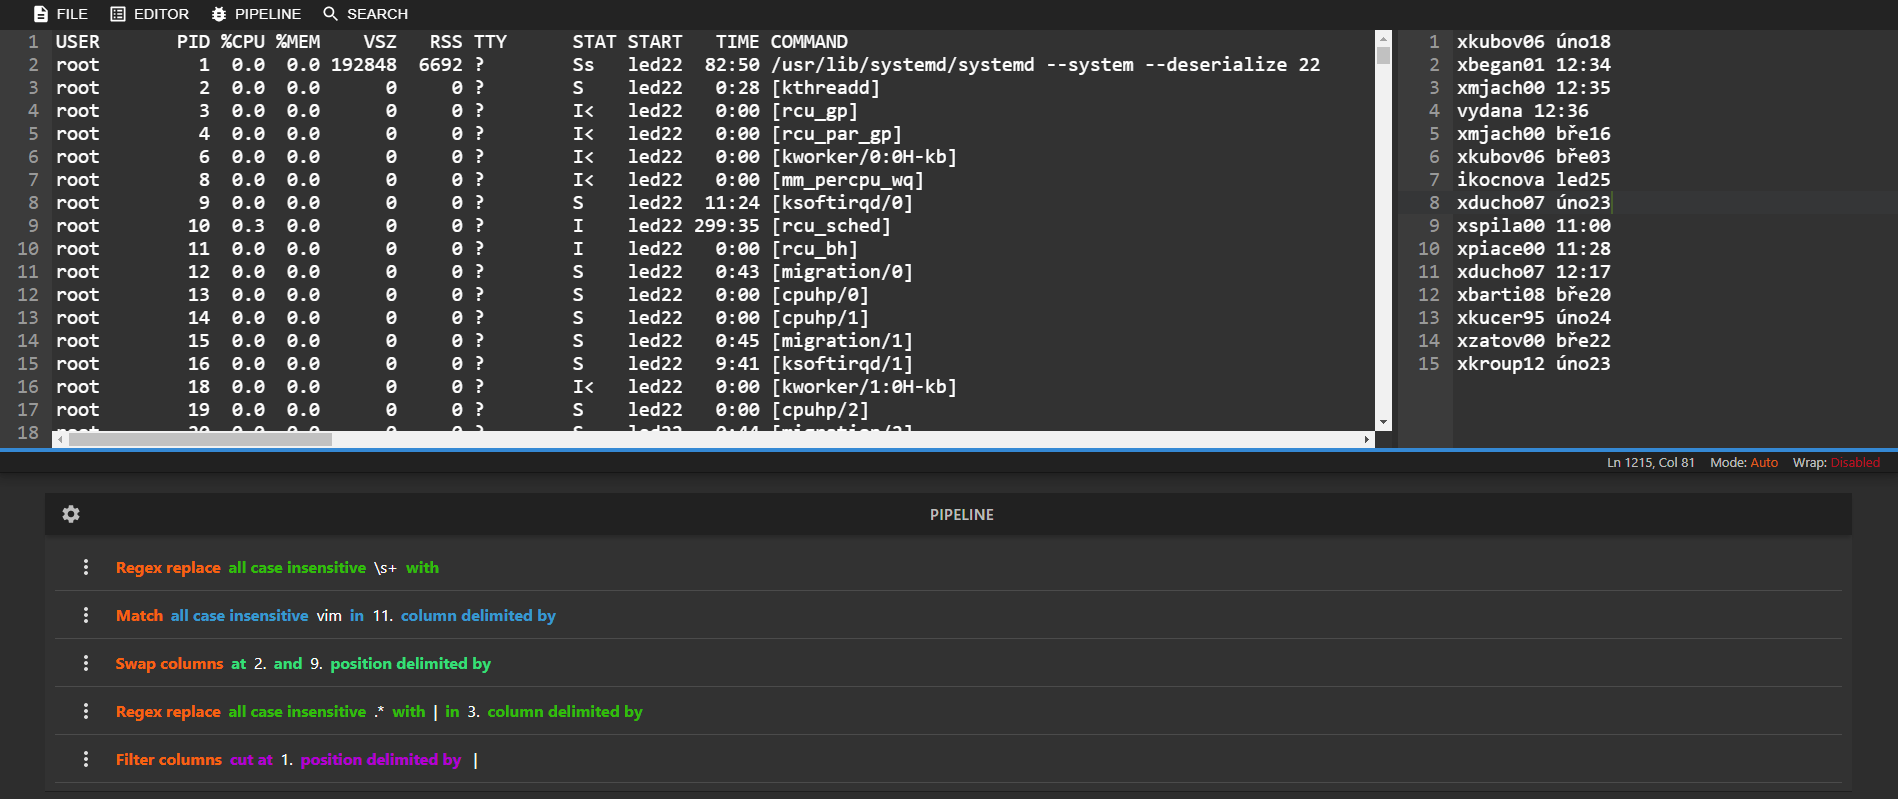
\includegraphics[width=1\textwidth]{obrazky-figures/Filtrace1.PNG}
	\caption{Filtrace uživatelů s~aktivní instancí textového editoru \texttt{vim} s~časovým údajem.}
	\label{obr:Filtrace1}
\end{figure}

\subsubsection*{Vygenerovaný ekvivalentní shell skript}
\begin{verbatim}
cat $FILENAME | sed -E 's/\s+/\ /gI' | awk -F '[ ]' -v OFS=' ' 
'{IGNORECASE=1} $11~/vim/' | awk -F '[ ]' -v OFS=' ' 
'{t=$2;$2=$9;$9=t;print;}' | awk -F '[ ]' -v OFS=' ' 
'{IGNORECASE=1}{gsub(".*", "|", $3); print }' | awk -F '|' '{print $1}'
\end{verbatim}

\subsection*{2. ukázka}
V tomto případě (viz obrázek~\ref{obr:Filtrace2}) byla data filtrována nad log souborem generovaný ovladačem prohlížeče při automatickém testování (viz fragment na výpisu~\ref{vyp:vstup2}). Z dat byly získány všechny unikátní chybové záznamy (viz fragment na výpisu~\ref{vyp:vystup2}).
\begin{lstlisting}[language=TeX, caption={Fragment vstupních dat.}, label={vyp:vstup2}]
1586875405783	mozrunner::runner	INFO	Running command: "/usr/bin/firefox" "-marionette" "-foreground" "-no-remote" "-profile" "/tmp/rust_mozprofileuOpWOb"
1586875406178	addons.webextension.doh-rollout@mozilla.org	WARN	Loading extension 'doh-rollout@mozilla.org': Reading manifest: Invalid extension permission: networkStatus
1586875406681	addons.webextension.screenshots@mozilla.org	WARN	Loading extension 'screenshots@mozilla.org': Reading manifest: Invalid extension permission: mozillaAddons
\end{lstlisting}

\begin{lstlisting}[language=TeX, caption={Fragment výstupních dat.}, label={vyp:vystup2}]
###!!! [Parent][DispatchAsyncMessage] Error: PLayerTransaction::Msg_ReleaseLayer Processing error: message was deserialized, but the handler returned false (indicating failure)
###!!! [Parent][RunMessage] Error: Channel closing: too late to send/recv, messages will be lost
Exiting due to channel error. 
\end{lstlisting}

\begin{figure}[hbt]
	\centering
	\setlength{\fboxsep}{0pt}
	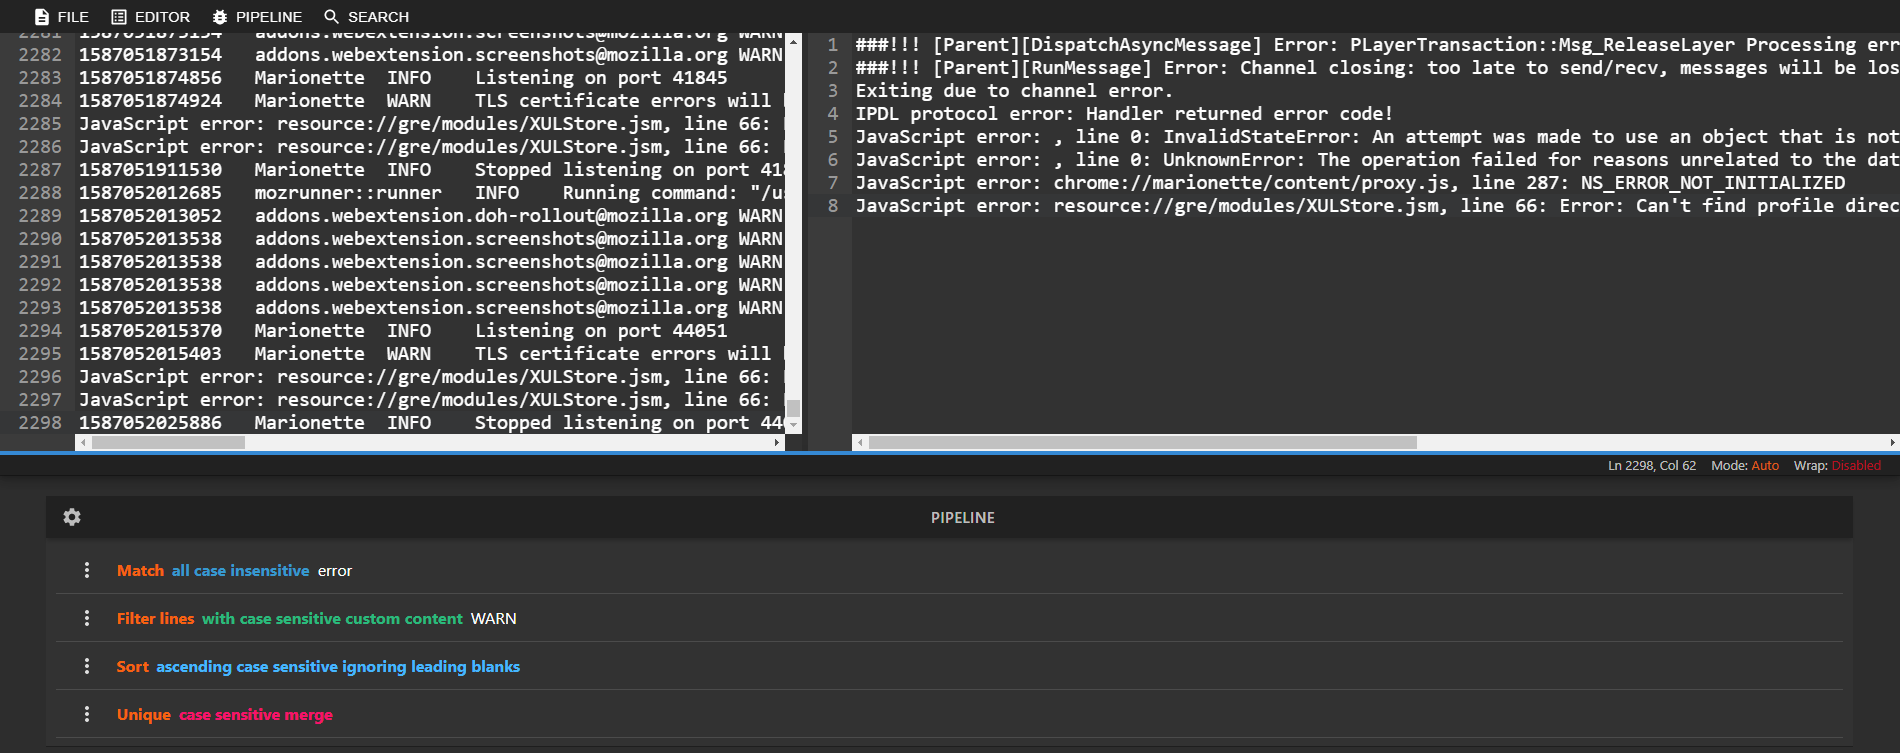
\includegraphics[width=1\textwidth]{obrazky-figures/Filtrace2.PNG}
	\caption{Filtrace chybových záznamů z~webového ovladače Gecko.}
	\label{obr:Filtrace2}
\end{figure}

\subsubsection*{Vygenerovaný ekvivalentní shell skript}
\begin{verbatim}
cat $FILENAME | grep -E -i 'error' | sed -E '/WARN/d' | 
LC_ALL=C sort -sb | uniq
\end{verbatim}

\section{Automatizované testování}
\label{sec:Automatické testování}
Kvůli častým změnám v~kódu nebo aktualizaci stromu závislostí byly implementovány automatizované testy, jejichž účelem bylo otestovat základní funkcionalitu aplikace a~případně upozornit na chyby, které by mohly vzniknout při nekompatibilitě. Výsledkem bylo ušetření velkého množství času, který by musel být vynaložen při manuálním testovaní mnou nebo jinými testery při opakujících se operacích s~každou novou verzí aplikace.

Testy \cite{website:BDD} byly napsány na metodice \textbf{behavior-driven development} (dále jen BDD), což umožňuje psát nebo číst průběh testů v~přirozeném jazyce i~uživateli, který nemusí disponovat znalostmi programování (např. analytik, stakeholder nebo koncový uživatel) a~tester poté tyto kroky implementuje. Testy jsou děleny na testovací případy, které se nazývají scénáře a~jsou napsány v~jazyce Gherkin\footnote{Gherkin: \url{https://cucumber.io/docs/gherkin/reference}}, který je strukturován v~pořadí kontext-akce-výsledek. Jeho účelem je srozumitelně popsat jakým způsobem by se měl daný objekt chovat v~různých situacích s~různými parametry. Tento scénář je pak uložen v~souboru se speciální formátem \texttt{.feature}, který je poté čitelný nástroji podporující BDD jako např. Cucumber, JBehave, Behat aj. Celkem bylo implementováno přes $500$~kroků ve více než $60$~scénářích.

\section{Uživatelské testování}
Během implementace probíhala konzultace se čtyřmi potenciálními uživateli aplikace (s~dalšími jen příležitostně), se kterými byla validována přehlednost uživatelského rozhraní. Uživatelé byli vybráni podle následujících kategorií:
\begin{itemize}
    \item \textbf{Technicky zdatný} -- Celkem 1 uživatel.
    \item \textbf{Technicky středně zdatný} -- Celkem 2 uživatelé.
    \item \textbf{Běžný uživatel} -- Celkem 1 uživatel.
\end{itemize}
Testování odhalilo několik chyb (bugů), které byly opraveny. Zejména se jednalo o~operace nad neočekávanými daty nebo o~problémy s~dynamikou webu, kdy se při určitém pořadí změn velikostí elementů měnila šířka obou editorů nebo po změně velikosti editoru a~následným změnám okna prohlížeče, zůstala pozice výstupního editoru statická, přestože by měl poměr zůstat zachovaný. Zároveň také vzniklo několik dalších požadavků a~nápadů, které byly z~velké části do aplikace ať už přímo nebo nepřímo implementovány. Takovým nápadem byl například popis funkčnosti nástrojů, společný vyhledávač, aj.

Zajímavým poznatkem z~testování byla skutečnost, že běžní uživatelé, kteří podobné nástroje neznají nebo nepoužívají, provádějí filtraci nad jednoduššími daty a~používají poměrně málo operací, naopak pokročilejší uživatelé s~odborněji zaměřenými daty provádějí více operací a~jejich požadavky na výstupy jsou velmi konkrétní. Největší problém v~orientaci bylo dělení nástrojů do kategorií. Každý uživatel měl jiný názor na jejich dekompozici ať už do počtu kategorií nebo jejich členění či jinak, bylo proto nutné najít optimální střední cestu, která každého zčásti uspokojila, přestože obsahovala pár kompromisů. Výsledný návrh poté neprokázal chaotické řešení a~uživatelé po rychlém prozkoumání těchto kategorií byli schopni plynule pracovat. Teorie k~názvům je potom následující:
\begin{itemize}
    \item \textbf{Find} -- Obsahuje nástroje, které vyberou záznamy podle zvolených kritérií. O výsledných záznamech pak lze s~jistotou říci, že obsahují právě tuto informaci.
    \item \textbf{Replace} -- Nástroje v~této kategorii jsou určeny pro náhradu části vstupního textu.
    \item \textbf{Reduce} -- V této kategorii jsou obsažený nástroje, které nějakým způsobem text redukují. O výsledných záznamech nemusíme mít konkrétní informaci, kterou nesou.
    \item \textbf{Modify} -- Zde jsou nástroje, které žádným způsobem text neredukují, ale modifikují nebo obohacují.
\end{itemize}

\subsection*{Měřený úkol}
Cílem poslední části testování bylo zjistit, s~jakou časovou efektivitou je uživatel schopen data vyfiltrovat oproti klasickému linuxovému skriptování v~shellu. Technicky zdatnému uživateli, jehož náplní práce není přímo tato problematika, přesto mu není úplně cizí, byla poskytnuta data, která musel následně transformovat do požadované podoby v~aplikaci (viz obrázek~\ref{obr:Filtrace3}), přičemž mu byl měřen čas. Poté jeho úkolem bylo provést tu stejnou transformaci nad stejnými daty v~shellu pomocí vyhledávače na internetu. Výsledné časy jsou zaznamenány v~tabulce~\ref{tab:Výsledné časy při testování}.

\subsubsection{Zadání}
Byl poskytnutý přístupový log soubor ze serveru, který obsahoval přes $21\,000$~záznamů (viz fragment na výpisu~\ref{vyp:vstup3}). Úkolem bylo vypsat všechny IP adresy, které poslali požadavek na server po datu 27.12.2015 (včetně), seznam adres musel být bez redundanci s~prefixem počtu přístupu dané adresy (viz fragment na výpisu~\ref{vyp:vystup3}).

\begin{lstlisting}[language=TeX, caption={Fragment výstupních dat.}, label={vyp:vstup3}]
109.169.248.247 - - [12/Dec/2015:18:25:11 +0100] "GET /administrator/ HTTP/1.1" 200 4263 "-" "Mozilla/5.0 (Windows NT 6.0; rv:34.0) Gecko/20100101 Firefox/34.0" "-"
109.169.248.247 - - [12/Dec/2015:18:25:11 +0100] "POST /administrator/index.php HTTP/1.1" 200 4494 "http://almhuette-raith.at/administrator/" "Mozilla/5.0 (Windows NT 6.0; rv:34.0) Gecko/20100101 Firefox/34.0" "-"
46.72.177.4 - - [12/Dec/2015:18:31:08 +0100] "GET /administrator/ HTTP/1.1" 200 4263 "-" "Mozilla/5.0 (Windows NT 6.0; rv:34.0) Gecko/20100101 Firefox/34.0" "-"
\end{lstlisting}

\begin{lstlisting}[language=TeX, caption={Fragment výstupních dat.}, label={vyp:vystup3}]
5 1.0.188.61
1 101.226.169.219
3 104.144.248.16
\end{lstlisting}

\begin{figure}[hbt]
	\centering
	\setlength{\fboxsep}{0pt}
	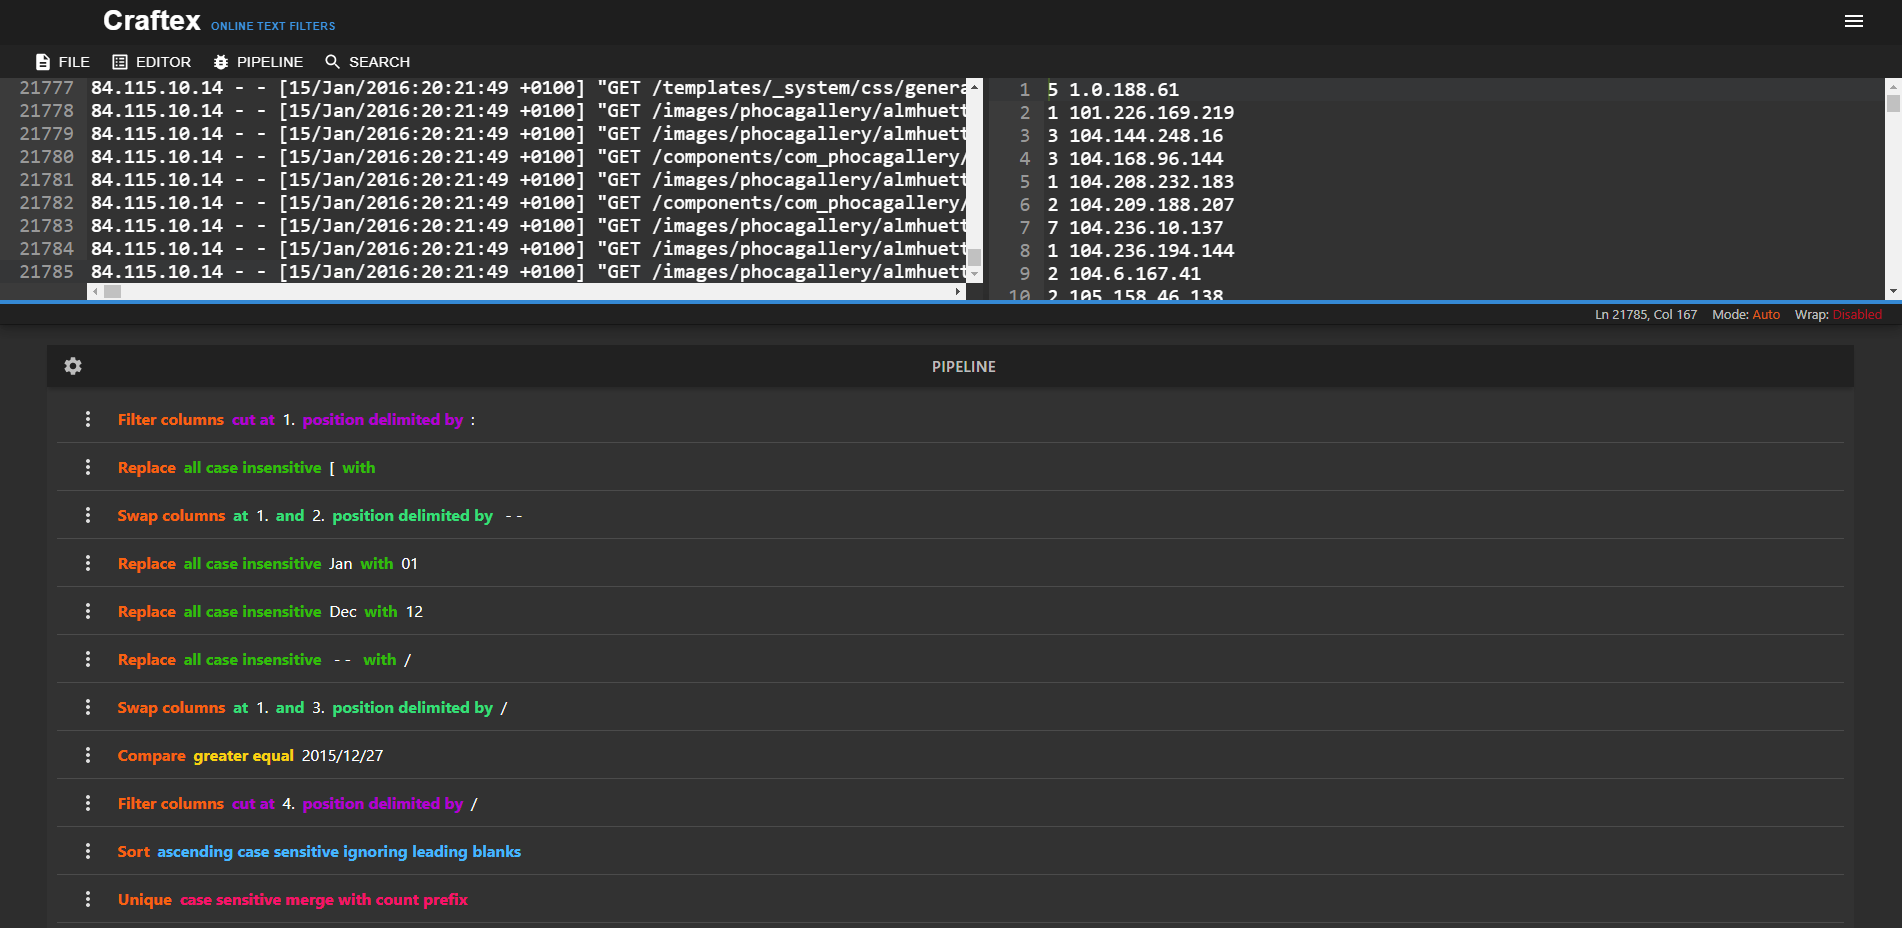
\includegraphics[width=1\textwidth]{obrazky-figures/testovaci_ukol.PNG}
	\caption{Výpis IP adres včetně počtu jejich přístupů na server po datu 27.12.2015 (včetně) z~přístupového log souboru.}
	\label{obr:Filtrace3}
\end{figure}

\subsubsection*{Vygenerovaný ekvivalentní shell skript}
\begin{verbatim}
cat $FILENAME | awk -F ':' '{print $1}' | sed -E 's/\[//gI' | 
awk -F ' - - ' -v OFS=' - - ' '{t=$1;$1=$2;$2=t;print;}' | 
sed -E 's/Jan/01/gI' | sed -E 's/Dec/12/gI' | sed -E 's/\ \-\ \-\ /\//gI' | 
awk -F '/' -v OFS='/' '{t=$1;$1=$3;$3=t;print;}' | 
awk -F '\n' '$1 >= "2015/12/27"' | awk -F '/' '{print $4}' | 
LC_ALL=C sort -sb | uniq -c | sed 's/^[[:blank:]]*//'
\end{verbatim}

\begin{table}[H]
    \centering
    \caption{Výsledné časy při testování}
    \label{tab:Výsledné časy při testování}
    \begin{tabular}{|c|c|c|}
        \hline
         & \textbf{Aplikace} & \textbf{Shell}  \\ \hline
        \textbf{Čas} & 11~minut 36~sekund & 1~hodina 6~minut 25~sekund \\ \hline
    \end{tabular}
\end{table}

\subsubsection{Doplňující otázky}
Po provedení úkolu byly uživateli položeny následující otázky, jejichž účelem je zhodnotit přínos aplikace a~poukázat na její výhody či nedostatky.
\begin{itemize}
    \item \textit{Narazil jste při práci na nějaké problémy? Případně změnil byste něco?} Uspořádání nástrojů by mohlo být podle abecedy, možná bych to pak vyhledal rychleji.
    \item \textit{Kdyby jste dostal podobné zadání na zpracování prostého textu, jak by jste tento problém řešil?} Nejspíše bych použil Excel, PlanMaker nebo případně bych data manuálně zpracoval, pokud by nebyla tak rozsáhlá.
    \item \textit{Čím Vás aplikace oslovila?} Přátelské rozhraní (hlavně vůči terminálu), data lze zpracovat bez znalostí funkcí oproti Excelu. Aplikaci bych i~znovu použil, ale záleží na objemu dat, jejich formátu a~operacích.
    \item \textit{Myslíte, že je v~aplikaci něco zbytečného nebo nadbytečného?} Nic mě nenapadá, dokážu si představit situace, ve kterých má každá funkcionalita svůj účel.
    \item \textit{Myslíte, že v~aplikaci něco schází?} Vždycky se dá něco vylepšit, teď by se mi zrovna hodilo řazení měsíců v~roce podle jejich názvu místo číselné hodnoty.
\end{itemize}

%=========================================================================
\chapter{Závěr}
Cílem této práce bylo navrhnout a~implementovat webový nástroj pro filtraci textu, který umožní uživatelům snadno a~efektivně zpracovat data s~možností prototypování a~ladění, který řeší danou problematiku jinak než doposud jiné internetové aplikace. Důležitou částí bylo aplikaci testovat nad vhodnými daty, prokázat tak její funkčnost a~odladit ji co nejvíce pro koncové uživatele.

V teoretické části byla nastíněna problematika filtrace, kde je možné se s~ní setkat a~byla provedena analýza dosavadních řešení. Následně bylo navrhnuto řešení této práce a~návrh rozhraní za pomoci interaktivní makety. Po volbě použitých technologií, zvážení alternativ a~následné implementaci vznikla funkční aplikace, která je schopna text plynule převádět, generovat nápomocné skripty a~nabízí nemalé množství nástrojů. Hlavním úspěchem je snadné ladění, které je realizováno na více místech aplikace, zejména v~oblasti pipeline dodatečnou manipulací, v~oblasti textu pomocí breakpointů nebo jiných funkcí, které aplikace nabízí. Nemalá část této práce byla věnována testování, během kterého byla pořízena testovací datová sada. V této fázi byly implementovány automatizované testy a~provedeno uživatelské testování, které se promítlo i~do výsledné podoby aplikace.

Pro budoucí rozšíření je možné aplikaci obohatit o~serverovou část, která umožní uživatelům zakládat účty, pod kterými budou moci své filtry ukládat a~sdílet pomocí odkazů. Další možností může být zavedení tipů pro zefektivňování řazení nástrojů (např. $2\times$ stejné otočení nemá na výsledek žádný efekt apod.).

Osobně mě práce obohatila o~zkušenosti všemi fázemi vývoje aplikace od návrhu, přes implementaci až po testování a~nasazení. Zejména část testování byla časově náročnější, než jsem původně očekával a~tuto znalost určitě uplatním v~budoucích projektech.
